\chapter{Исследование производительности систем радиочастотной идентификации}\label{ch:ch2}

В настоящей главе исследуется возможность использования технологии пассивной радиочастотной идентификации стандарта EPC Gen-2 \cite{StdGen2} для идентификации автотранспорта, движущегося со скоростями порядка 60 "--- 150 км/ч. Сначала, в разделе \ref{sec:ch2_structure}, будут описаны компоненты системы радиочастотной идентификации автомобилей, а в разделе \ref{sec:ch2_general_scheme} также в наиболее общей форме приведены зависимости, определяющие вероятность успешной идентификации подвижной метки. Эта вероятность зависит от числа раундов, в которых метка успевает принять участие, а также от вероятности идентификации в каждом из раундов. Для анализа факторов, от которых зависит число раундов, в разделе \ref{sec:ch2_durations} будут исследованы зависимости длительностей команд, ответов и раундов от различных параметров протокола, а для анализа вероятности идентификации метки в каждом из раундов в разделе \ref{sec:ch2_channel} будет приведена модель радиоканала, учитывающая особенности многолучевого распространения сигналов вблизи дороги, зависимость мощности отраженных сигналов от материала поверхности дороги, а также влияние эффекта Доплера, и будут получены оценки вероятностей битовых ошибок (BER) при передаче ответов меток. С учетом сделанных расчетов будет уточнено определение области, в которой метки имеют возможность передать свои идентификаторы считывателю, и будет сделан аналитический расчет вероятности идентификации метки. В разделе \ref{sec:ch2_sim} кратко описывается имитационная модель, а в разделе \ref{sec:ch2_results} приводятся результаты моделирования системы радиочастотной идентификации автомобилей. Раздел \ref{sec:ch2_conclusion} завершает главу. В следующей главе будет приведена аналитическая модель, позволяющая более точно оценить влияние сбросов питания и смены флагов опроса на вероятность идентификации.

Результаты, представленные в главе, были опубликованы в журналах \cite{RFID_JRFID2017,QS_TCOMM2012,QS_JITCS2013}, сборниках, индексируемых Scopus/WoS \cite{RFID_IEEERFID2017,RFID_DCCN2016_CCIS,RFID_SYNCHROINFO2018}, и представлены в трудах конференций \cite{Fedotov2020, Fedotov2020a, RFID_DCCN2015_RUS,RFID_DCCN2013_RUS}.





%%%%%%%%%%%%%%%%%%%%%%%%%%%%%%%%%%%%%%%%%%%%%%%%%%%%%%%%%%%%%%%%%%%%%%%%%%%%%%%%
\section{Структура системы радиочастотной идентификации} \label{sec:ch2_structure}
%%%%%%%%%%%%%%%%%%%%%%%%%%%%%%%%%%%%%%%%%%%%%%%%%%%%%%%%%%%%%%%%%%%%%%%%%%%%%%%%
Система радиочастотной идентификации автомобилей состоит из RFID-считывателя и RFID-меток (радиометок), размещенных на автомобилях (см. рис.~\ref{fig:ch2_system_structure}). Метки и считыватель работают по стандарту EPC Class 1 Generation 2 \cite{StdGen2}

\begin{figure}[ht]
  \centerfloat{
    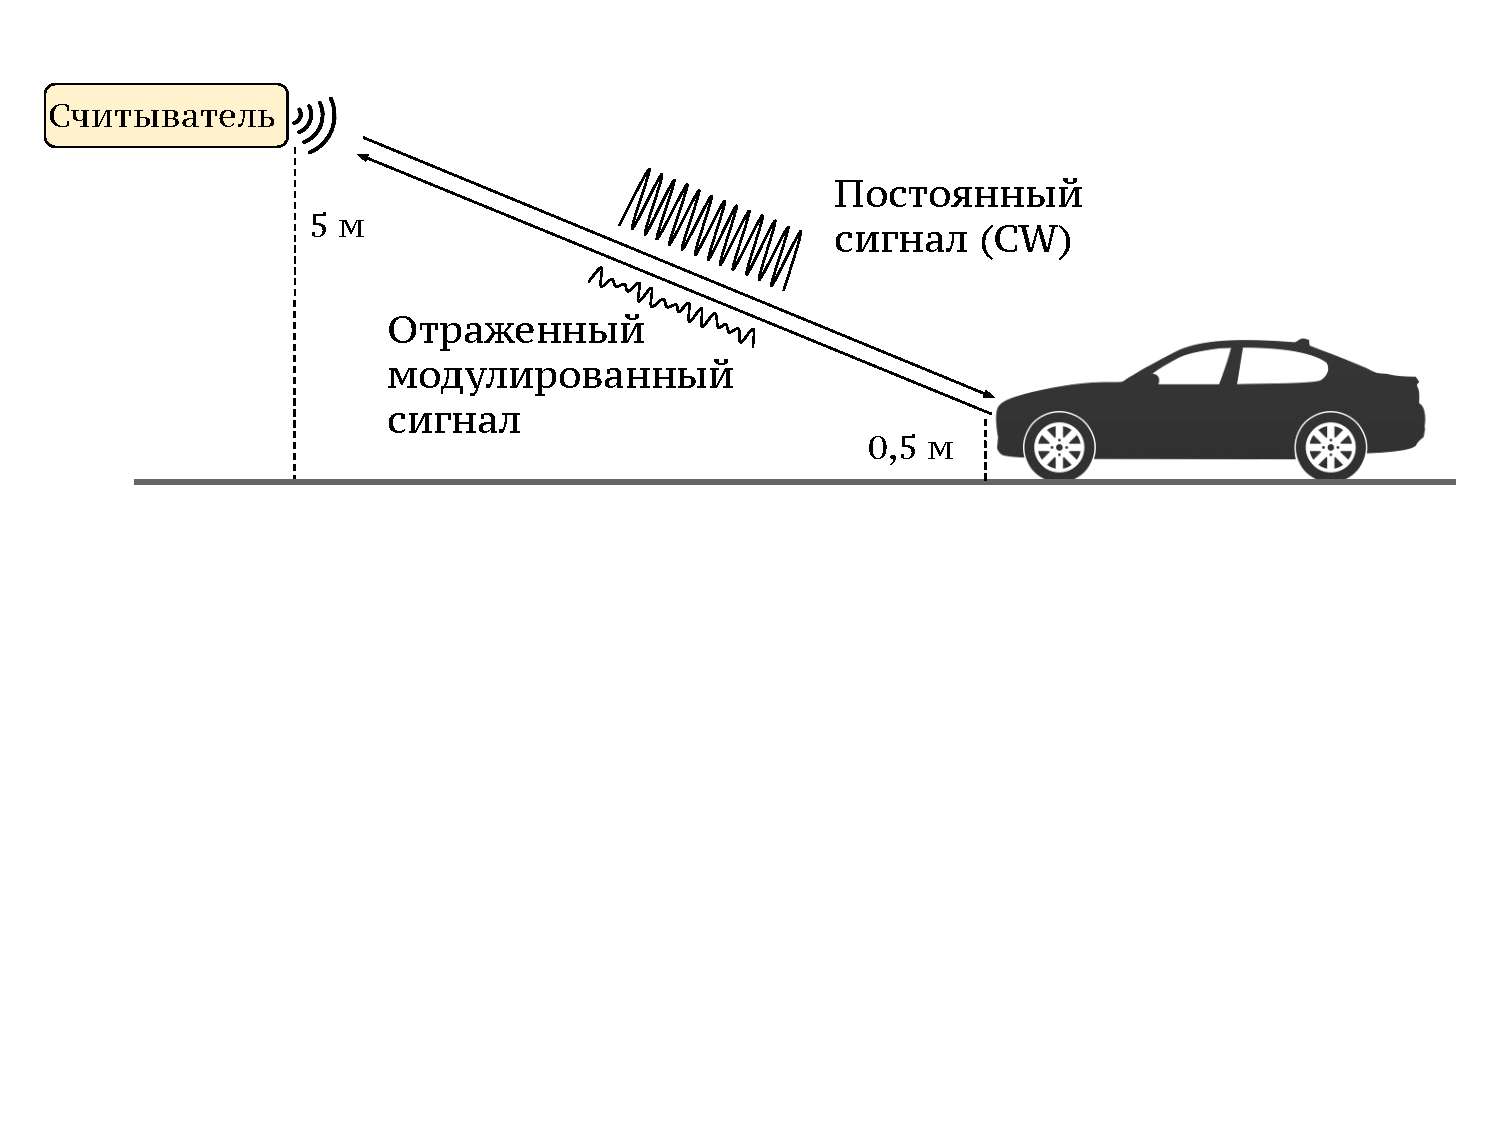
\includegraphics [scale=0.5] {chapter2/ch2_system_structure}
  }
  \caption{Структура системы радиочастотной идентификации автомобилей}
  \label{fig:ch2_system_structure}
\end{figure}

Метки могут размещаться на регистрационных номерных знаках, под лобовым стеклом или на корпусе автомобиля. В настоящей работе рассматривается случай, когда метки расположены на номерах, поскольку этот вариант был использован в проведенном в г. Казань эксперименте. Кроме того, размещение меток в номерных знаках обладает рядом преимуществ: расположение знаков относительно дорожного полотна варьируется в малых пределах, зона номерного знака не загорожена никакими проводящими поверхностями, наконец это решение можно в дальнейшем легко стандартизировать и масштабировать за счет монтирования меток в выпускаемые номерные знаки.

RFID-считыватель размещается над дорогой (например, на тех же опорах, на которых сегодня размещаются камеры), на высоте приблизительно 5 метров; считыватель может оснащаться от 1 до 4 антенн. Таким образом, один считыватель может читать метки в передних и задних номерах на двухполосной дороге.

Связь между меткой и считывателем возможна при соблюдении двух условий: метка получает достаточно энергии для работы и декодирования команд от считывателя (чувствительность современных меток имеет порядок -18 дБм), и отраженный модулированный меткой сигнал поступает на считыватель на достаточно высокой мощности, чтобы быть успешно распознанным и декодированным (при отсутствии коллизий, уровень принимаемого сигнала для современных считывателей должен быть не ниже минус 80 дБм). На практике это означает, что дальность связи составляет порядка 8 -- 15 метров. Однако, из-за особенностей распространения сигнала вблизи автодороги, область, в которой метка может получить достаточно энергии, может иметь достаточно сложный вид и состоять из нескольких непересекающихся областей, общая ширина которых может составлять 2 -- 3 метра. Подробнее эти эффекты будут рассмотрены в последующих разделах.



%%%%%%%%%%%%%%%%%%%%%%%%%%%%%%%%%%%%%%%%%%%%%%%%%%%%%%%%%%%%%%%%%%%%%%%%%%%%%%%%
\section{Общая схема расчёта вероятности идентификации автомобилей}\label{sec:ch2_general_scheme}
%%%%%%%%%%%%%%%%%%%%%%%%%%%%%%%%%%%%%%%%%%%%%%%%%%%%%%%%%%%%%%%%%%%%%%%%%%%%%%%%
Производительность системы определяется как доля успешно идентифицированных автомобилей. Полагая, что успешного чтения хотя бы одной метки достаточно для идентификации автомобиля, вероятность идентификации можно описать следующим образом:

$$
	\mathbb{P}\{A_x\} = 1 - \prod\limits_{\forall t \in  \mathfrak{T}_x} (1 - \mathbb{P}\{A_t\}),
$$
где $A_x$ "--- событие идентификации автомобиля $x$, $A_t$ "--- событие идентификации метки $t$, а $\mathfrak{T}_x$ есть множество меток, размещенных на автомобиле $x$. Вероятность идентификации метки $\mathbb{P}\{A_t\}$ зависит от длительности раунда инвентаризации, вероятности успешной передачи ответа и числа меток в области чтения:

$$
	\mathbb{P}\{A_t\} = 1 - (1 - (1 - \mathbb{P}\{A_c\})\mathbb{P}\{A_r\})^{N_r},
$$
где $A_c$ "--- событие возникновения коллизии, $A_r$ "--- событие успешной передачи меткой ее идентификатора и $N_r$ "--- число раундов, в которых метка успевает принять участие.

Пусть $N_t$ "--- число меток в области чтения и $Q$ "--- параметр антиколлизионного протокола. \cite{StdGen2}. Тогда вероятность возникновения коллизии для данной метки определяется следующей формулой:

$$
	\mathbb{P}\{A_c\} = 1 - (1 - 2^{-Q})^{|N_t| - 1}.
$$

Число раундов можно грубо оценить как:

$$
	N_r \approx \frac{D_r}{v}\cdot\frac{1}{T_r},
$$
где $D_r$ "--- общая длина участка дороги с хорошими условиями для чтения (т.е. на этом участке метка получает достаточно энергии для работы и битовая ошибка достаточно низка), $T_r$ "--- средняя длина раунда при заданном числе меток и параметрах протокола, $v$ "--- скорость движения метки. В действительности количество раундов представлеяет собой случайную величину, зависящую от множества параметров, включая количество меток в области чтения, настройки протокола, непосредственный выбор метками слотов для ответов (определяет количество коллизий, пустых слотов и слотов с ответами). Также число раундов зависит от результатов попыток передачи меткой её идентификатора, а также от того, сбрасывал ли считыватель питание между раундами "--- влияние этих факторов оказывается очень существенным и исследуется подробнее в следующей главе диссертации.

Согласно \cite{Nikitin2008}, при отсутствии коллизий основным источником ошибок при расчете $\mathbb{P}\{A_r\}$ является высокий BER при приеме ответов от меток. Пусть $r$ "--- ответ метки, $\mathfrak{R}$ "--- множество всех ответов метки, передача которых необходима для успешной идентификации. Обозначая битовую длину ответа как $|r|$, вероятность успешной передачи всех ответов $\mathbb{P}\{A_r\}$ метки можно вычислить по формуле:

$$
	\mathbb{P}\{A_r\}=\prod_{r \in \mathfrak{R}}(1-B)^{|r|}.
$$

Множество $\mathfrak{R}$ обязательно содержит ответ RN16 на команду, с которой начался слот, в котором метка передаёт ответ (Query, QueryRep или QueryAdjust) и ответ на команду ACK (PC+EPC+CRC). Если для идентификации метки также используется 64-битное значение из банка TID, то $\mathfrak{R}$ также включает ответы на Req\_RN и Read.

Из приведенных формул видно, что для максимизации вероятности идентификации автомобиля необходимо увеличивать вероятность успешной передачи меткой ответов и число раундов, и одновременно уменьшать вероятность коллизий. Однако эти требования вступают в противоречие: более низкий BER достигается при более надежных и медленных настройках протокола, а вероятность коллизии снижается при росте числа слотов, но все это ведет к увеличению длительности раунда. В последующих разделах будет разработан комплекс моделей, позволяющий проанализировать вероятность идентификации метки при различных допущениях, а в конце главы будут приведены результаты расчета вероятности идентификации автомобиля при различных настройках протокола и скорости движения, полученные с помощью детализированной имитационной модели.







%%%%%%%%%%%%%%%%%%%%%%%%%%%%%%%%%%%%%%%%%%%%%%%%%%%%%%%%%%%%%%%%%%%%%%%%%%%%%%%%
\section{Анализ влияния параметров протокола на длительности раундов}\label{sec:ch2_durations}
%%%%%%%%%%%%%%%%%%%%%%%%%%%%%%%%%%%%%%%%%%%%%%%%%%%%%%%%%%%%%%%%%%%%%%%%%%%%%%%%
Считыватель использует модуляции DSB-ASK, SSB-ASK и PR-ASK, а в качестве схемы кодирования используется PIE. Из-за использования PIE (Pulse Interval Encoding) длительность передачи команды зависит от её содержания, так как длительности символов data\_0 и data\_1 отличаются в 1,5--2 раза. Перед каждой командой Query считыватель передает преамбулу, а перед остальными "--- более короткую синхронизирующую последовательность. В таблице \ref{table:ch2_commands_and_replies_durations} показаны длительности команд и ответов для некоторых настроек протокола. Параметры Tari, TRcal, QUERY и PC+EPC+CRC заданы в микросекундах, BLF "--- в килогерцах, а M выражает число символов на бит в ответе метки (порядок кода Миллера, используемого меткой).

\begin{table}[!t]
	\renewcommand{\arraystretch}{1.3}
	\caption{Длительности команд и ответов при разных настройках протокола.
	Длительности QUERY and PC+EPC+CRC даны в микросекундах.}
	\label{table:ch2_commands_and_replies_durations}
	\centering
	\begin{tabular}{|c|c|c|c|c|c|c|}
		\hline
		DR   & Tari & TRcal & BLF   & M & QUERY & PC+EPC+CRC  \\\hline
		64/3 & 6.25 & 33.38 & 639.2 & 1 & 252.13 & 211.2      \\\hline
		64/3 & 6.25 & 33.38 & 639.2 & 8 & 270.88 & 1739.67    \\\hline
		64/3 & 12.5 & 66.75 & 319.6 & 1 & 491.75 & 422.4      \\\hline
		64/3 & 25.0 & 133.5 & 159.8 & 1 & 971.0  & 844.8      \\\hline
		64/3 & 25.0 & 225.0 & 94.81 & 1 & 1062.5 & 1423.83    \\\hline
		8    & 6.25 & 33.38 & 239.7 & 1 & 245.8  & 563.2      \\\hline
		8    & 25.0 & 225.0 & 33.56 & 8 & 1112.5 & 31275.0    \\\hline
	\end{tabular}
\end{table}

\begin{figure}[!t]
  \centerfloat{
    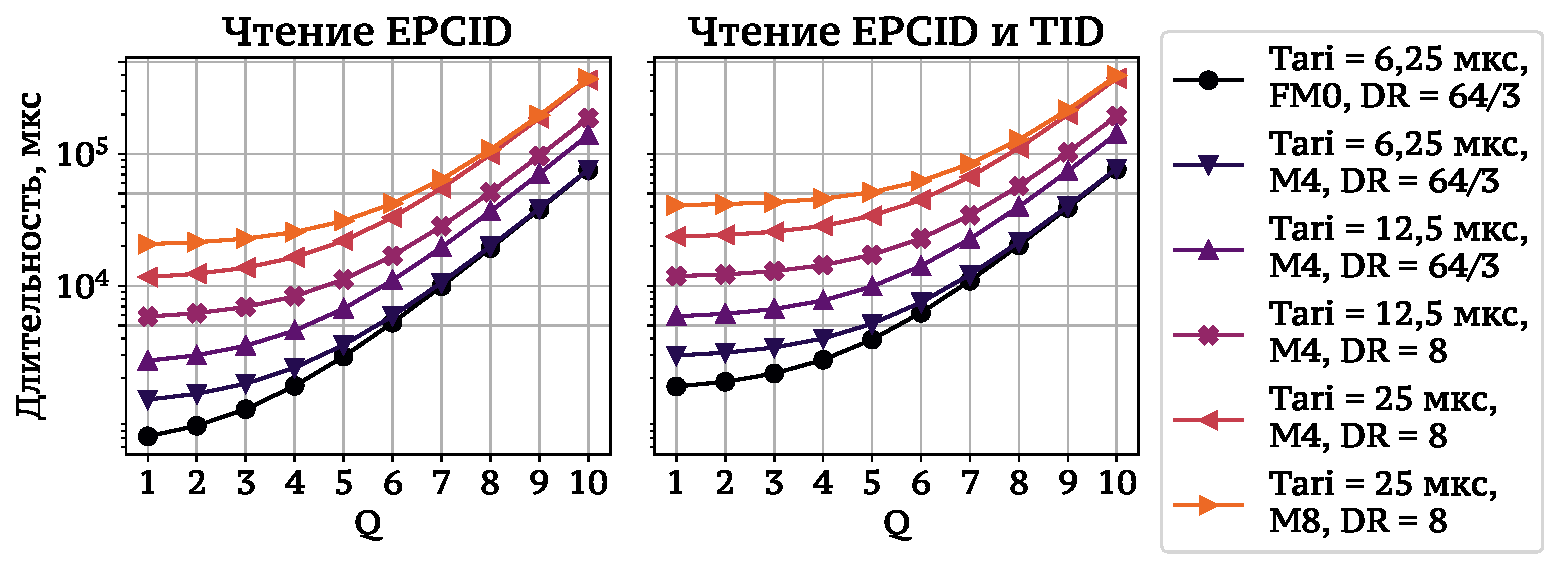
\includegraphics[width=3.3in]{chapter2/ch2_round_durations}
  }
	\caption{Зависимость максимальной длительности раунда от значения Q.}
	\label{fig:ch2_round_durations}
\end{figure}

\begin{figure}[!t]
	\centerfloat{
    \includegraphics[width=3.3in]{chapter2/ch2_round_numbers}
  }
	\caption{Зависимость максимального числа раундов, в которых принимает участние метка, от значения Q.}
	\label{fig:ch2_round_numbers}
\end{figure}


Выбор значений DR, Tari, M и TRcal значительно влияет на длительности команд и ответов. Так, длительность команды Query может варьироваться от 200~мкс до 1,1~мс, а длительность ответа PC+EPC+CRC на команду ACK "--- от 211~мкс до 31,2~мс (см. табл.~\ref{table:ch2_commands_and_replies_durations}).

При идентификации метки может использоваться только EPCID или комбинация EPCID и значений из других банков, например "--- TID. Первый вариант менее надежен, однако существенно быстрее второго "--- на чтение банков памяти требуется значительно больше времени, так как при этом необходимо осуществить дополнительный обмен сообщениями. На длительность идентификации также влияет, например, использование команды Select для настройки флагов меток и выбора популяции для опроса. В дальнейшем будем рассматривать два самых простых сценария: идентификацию меток только по EPCID (в этом случае взаимодействие ограничивается инвентаризацией) и по комбинации EPCID + TID. Кроме того, будем предполагать, что считыватель не использует команды QueryAdjust и не изменяет выбранное значение параметра Q.

На рис.~\ref{fig:ch2_round_durations} показана максимальная длительность раунда от значения Q, а на рис.~\ref{fig:ch2_round_numbers} "--- максимальное число раундов. Необходимо отметить, что реальная длина раунда может существенно отличаться в зависимости от того, сколько меток в нем отвечает успешно, сколько коллизий происходит и сколько слотов остаются пустыми. Однако, приведенные графики дают возможность увидеть различие в длительностях при использовании разных способов идентификации, а также зависимость от некоторых важных параметров протокола.









%%%%%%%%%%%%%%%%%%%%%%%%%%%%%%%%%%%%%%%%%%%%%%%%%%%%%%%%%%%%%%%%%%%%%%%%%%%%%%%%
\section{Моделирование радиоканала между считывателем и меткой}\label{sec:ch2_channel}
%%%%%%%%%%%%%%%%%%%%%%%%%%%%%%%%%%%%%%%%%%%%%%%%%%%%%%%%%%%%%%%%%%%%%%%%%%%%%%%%
Для передачи данных от метки используется модуляция обратного рассеяния, метка (не оснащенная источником питания) не может усилить отраженный сигнал. Из-за этого мощность сигнала, принятого на стороне считывателя, значительно ниже, чем мощность на стороне метки. По этой причине битовая ошибка (BER) оказывается выше на стороне считывателя, то есть ошибки с гораздо большей вероятностью появляются при приеме ответов от метки, чем команд от считывателя. Значение BER на стороне считывателя оказывает существенное влияние на успешность чтения меток, поэтому это значение должно быть аккуратно рассчитано.

Для анализа BER рассчитаем бюджет соединения и полуичм значение сигнал--шум (SNR). Результаты этого расчета для стационарного считывателя и метки, размещенной на переднем номере автомобиля, двигающегося со скоростью 60~км/ч, приведены на рис.~\ref{fig:ch2_link_budget}. На горизонтальной оси всех графиков показано расстояние между передатчиком и приемником, на вертикальной "--- время, прошедшее с момента достижения волной приемника. Как будет показано далее (см. формулу~\eqref{eq:ch2_pathloss} для вычисления потерь на распространении сигнала), выбор значения скорости движения существенно влияет на скорость изменения величины затухания в заданной точке.

\begin{figure}[!t]
  \centerfloat{
    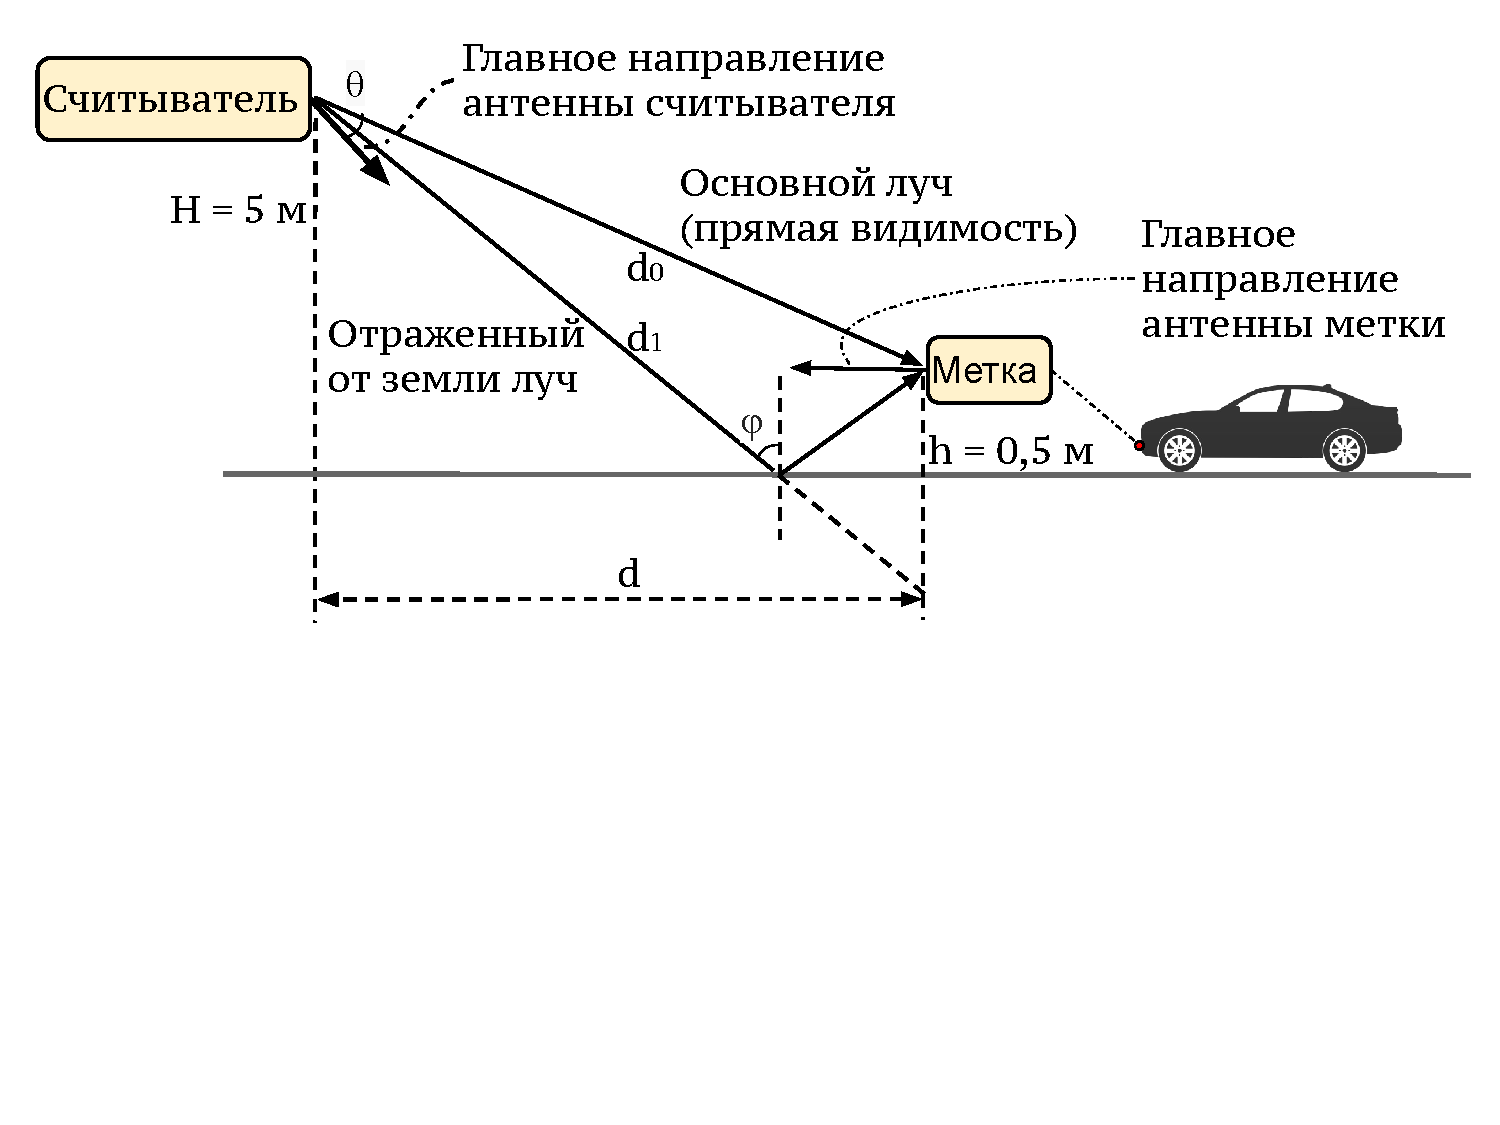
\includegraphics[width=\linewidth]{chapter2/ch2_geometry}
  }
	\caption{Схема системы радиочастотной идентификации автомобилей и ее геометрические параметры.}
	\label{fig:ch2_geometry}
\end{figure}



%%% --------------------------------------------
\subsection{Расчёт бюджета соединений}
%%% --------------------------------------------
Пусть $P_t^{(r)}$ "--- излучаемая мощность считывателя, $G^{(r)}$ "--- усиление антенны считывателя. Тогда эффективная изотропная излучаемая мощность (EIRP) составит $EIRP =  P_t^{(r)} G^{(r)}$. Здесь и далее надстрочный индекс используется для обозначения устройства: (r) для считывателя и (t) для метки; подстрочный индекс используется для обозначения направления передачи (прием или передача сигнала). При распространении сигнала от считывателя к метке сигнал испытывает затухание $A_{pl}^{(d)}$, зависящее от состояния радиоканала и взаимного расположения считывателя и метки друг относительно друга. Антенны устройств могут иметь различную поляризацию, что ведет к дополнительным потерям $A_{pol}$. Пусть усиление антенны метки равно $G^{(t)}$. Тогда мощность сигнала, принимаемого меткой, равна:

$$
	P_r^{(t)} = P_t^{(r)} G^{(r)} A_{pl}^{(d)} A_{pol} G^{(t)}.
$$

Если эта мощность меньше чувствительности метки $P_s^{(t)}$, то метка не включится и не сможет взаимодействовать со считывателем. В противном случае метка сможет передавать свои ответы за счет модулирования отраженного сигнала, мощность которого будет равна $P_t^{(t)}$. Поскольку при этом возникают дополнительные энергетические потери (например, из-за модуляции), равные $A_{bs}$, то мощность принятого и отраженного сигналов связаны как $P_t^{(t)} = P_r^{(t)} + A_{bs}$.

Для мощности сигнала, принятого от метки считывателем, можно написать следующее соотношение:

$$
	P_r^{(r)} = P_r^{(t)} G^{(t)} A_{bs} A_{pl}^{(r)} A_{pol} G^{(r)}.
$$

В общем случае потери на прямом (от считывателя к метке) и обратном (от метки к считывателю) путях могут отличаться. Это происходит из-за различия в поляризации (обычно на считывателях используются антенны с круговой поляризацией, а на метках "--- с линейной) и, как следствие, в коэффициенте отражения от земли.

\begin{table}[!t]
	\renewcommand{\arraystretch}{1.3}
	\caption{Параметры, использованные при расчете бюджета соединения}
	\label{table:ch2_budget_params}
	\centering
	\begin{tabular}{|c|c|}
		\hline
		Мощность, излучаемая считывателем, $P_t^{(r)}$ & 31.5~дБм\\
		\hline
		Усиление антенны считывателя, $G^{(r)}$ & 8~дБи\\
		\hline
		Усиление антенны метки, $G^{(t)}$ & 2~дБи\\
		\hline
		Чувствительность метки, $P_s^{(t)}$ & -18~дБм\\
		\hline
		Потери на поляризации, $A_{pol}$ & -3~дБ\\
		\hline
		Потери на модуляции на метке, $A_{bs}$ & -10~дБ\\
		\hline
		Потери в кабеле, $A_{bs}$ & -2~дБ\\
		\hline
	\end{tabular}
\end{table}

В дальнейших расчетах бюджета соединения будут использованы значения, приведенные в таблице~\ref{table:ch2_budget_params}, типичные для оборудования, применяемого в идентификации автомобилей. При расчете также следует учитывать потери в кабеле, соединяющем антенну со считывателем. Далее считается, что антенны считывателя имеют круговую поляризацию, а меток "--- линейную, таким образом потери на поляризации составляют -3~дБ.

\begin{figure}[!t]
	\centerfloat{
    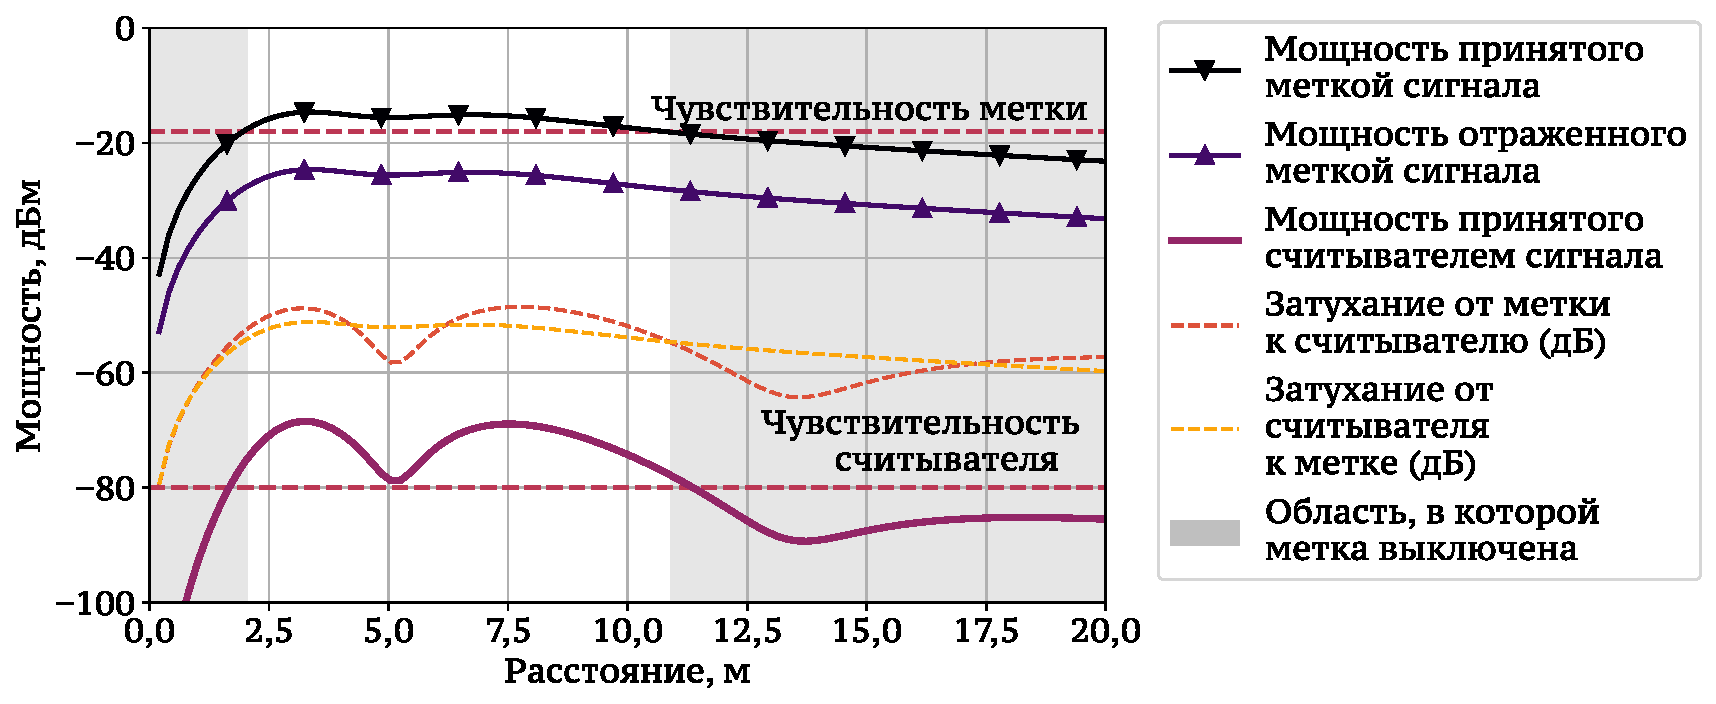
\includegraphics[width=3.3in]{chapter2/ch2_link_budget}
  }
  \caption{Расчет бюджета соединения в зависимости от расстояния между считывателем и меткой.}
  \label{fig:ch2_link_budget}
\end{figure}

На рис.~\ref{fig:ch2_link_budget} показан расчет мощностей сигналов, принятых и переданных меткой, принятого считывателем сигнала, а также величина затухания. Все кривые убывают немонотонно из-за изменений с расстоянием в коэффициентах отражения от земли, а также из-за влияния диаграмм направленности антенн (особенно сильно диаграмма направленности влияет на сигнал при близком расположении метки и считывателя, так как даже небольшое изменение расстояния ведет к ощутимому изменению в угле падения). Поскольку метка может работать только в тех областях, где принятый ею сигнал превышает чувствительность, графики мощностей передаваемого меткой и принимаемого считывателем сигнала лежат выше нуля только на ограниченном интервале.

На рис.~\ref{fig:ch2_heatmap_pathloss} показана величина потери из-за затухания сигнала при распространении от считывателя к метке (картина для обратного канала отличается незначительно), а на рис.~\ref{fig:ch2_heatmap_tag_rx_power} показан результат расчета мощности сигнала, принятого меткой. Для того, чтобы связь между расстоянием от считывателя до метки и временем при постоянной скорости оставалась линейной, в качестве расстояния рассматривается дистанция от опоры, на которой размещен считыватель, до метки, измеренная вдоль дороги (см. величину $d$ на рис.~\ref{fig:ch2_geometry}). Значительное влияние на результат расчета оказывает эффект Доплера, подробнее о котором будет рассказано в следующем разделе. Фактически из-за этого эффекта канал становится зависимым от времени, то есть при проезде через одну и ту же точку двух одинаковых меток в разное время принятая ими (а, соответственно, и отраженная) мощность будет различаться.


%    \centerfloat{
%        \hfill
%        \subcaptionbox[List-of-Figures entry]{Первый подрисунок\label{fig:knuth_2-1}}{%
%            \includegraphics[width=0.25\linewidth]{knuth1}}
%        \hfill
%        \subcaptionbox{\label{fig:knuth_2-2}}{%
%            \includegraphics[width=0.25\linewidth]{knuth2}}
%        \hfill
%        \subcaptionbox{Третий подрисунок, подпись к которому
%        не~помещается на~одной строке}{%
%            \includegraphics[width=0.3\linewidth]{example-image-c}}
%        \hfill
%    }
%    \legend{Подрисуночный текст, описывающий обозначения, например. Согласно
%    ГОСТ 2.105, пункт 4.3.1, располагается перед наименованием рисунка.}
%    \caption[Этот текст попадает в названия рисунков в списке рисунков]{Очень
%    длинная подпись к второму изображению, на~котором представлены две
%    фотографии Дональда Кнута}\label{fig:knuth_2}

\begin{figure}[ht]
  \centerfloat{
    \hfill
    \subcaptionbox{Затухание сигнала при распространении от считывателя к метке, дБ\label{fig:ch2_heatmap_pathloss}}{%
      \includegraphics[width=0.30\linewidth]{chapter2/ch2_heatmap_pathloss}
    }
    \hfill
    \subcaptionbox{Мощность принятого на метке сигнала, дБм\label{fig:ch2_heatmap_tag_rx_power}}{%
      \includegraphics[width=0.30\linewidth]{chapter2/ch2_heatmap_tag_rx_power}
    }
    \hfill
    \subcaptionbox{Битовая ошибка (BER) на считывателе\label{fig:ch2_heatmap_ber}}{%
      \includegraphics[width=0.30\linewidth]{chapter2/ch2_heatmap_ber}
    }
  }
  \legend{На горизонтальных осях показано расстояние от точки крепления считывателя до метки вдоль дороги (см. величину $d$ на рис.~\ref{fig:ch2_geometry}). На вертикальных осях показано время от начала приема меткой сигнала. Из-за эффекта Доплера канал меняется со временем, т.е. метки, расположенные на автомобилях, проезжающих через одну и ту же точку в разное время, застают канал в разных состояниях и получают сигналы разной мощности.}
  \caption{Расчет бюджета соединений и BER}
  \label{fig:ch2_heatmap}
\end{figure}




%%% --------------------------------------------
\subsection{Расчёт мощности принятых сигналов}
%%% --------------------------------------------

При движении меток и считывателей с ненулевой скоростью друг относительно друга сигналы оказываются подверженными эффекту Доплера, проявляющемуся в сдвиге частоты сигнала на величину, называемую доплеровским сдвигом, и равную:

$$
	\alpha = 1 - \frac{\upsilon \cos{\psi}}{c+\upsilon \cos{\psi}},
$$
где $c$ "--- скорость света, $\upsilon$ "--- скорость приёмника относительно передатчика, в роли приёмника может выступать как метка, так и считыватель (при этом их скорости будут иметь одинаковую величину и противоположные знаки), $\psi$ "--- угол между волновым вектором $\bm{k}$ и направлением движения, $f_c$ "--- несущая частота.

Для узкополосного сигнала в RFID-канале смещённую частоту можно приблизить выражением $\alpha f \approx f - \frac{\upsilon}{c}\cos{\psi} \cdot f_c = f - \nu$, где $\nu$ "--- доплеровский сдвиг:

$$
	\nu = \frac{\upsilon}{c} f_c\cos{\psi} = \frac{1}{2\pi}(\bm{\upsilon},\bm{k})
$$

При распространении сигнала он может отражаться от дороги, инженерных конструкций, других автомобилей и прочих объектов, то есть в моделируемой системе имеет место многолучевое распространение сигнала. При этом возникает множество копий сигнала $s(t)$, каждая из которых испытывает собственное затухание $h_i$, задержку $\tau_i$ и доплеровский сдвиг $\nu_i$, поскольку каждая копия распространяется по собственному пути, с которым, помимо длины, связаны углы передачи и приема сигнала. Пусть в сигнале присутствует прямая компонента (Line-of-Sight, LoS) сигнала и $N$ отраженных компонент (или лучей). Без потери общности рассуждений будем считать, что LoS-компонента описывается нулевым лучём, а отраженные компоненты "--- лучами $1 \dots N$. Принятый сигнал определяется следующей формулой:

\begin{equation}
	r(t) = \sum\limits_{i=0}^{N} h_i s(t-\tau_i) e^{j\nu_i t},
	\label{eq:ch2_rx_signal}
\end{equation}

Затухание $h_i$ может быть рассчитано как $h_i=\lambda/(4\pi d_i)R_i\Gamma_i$, где $\lambda$ "--- длина волны, $d_i$ "--- длина пути для $i$--го луча, $R_i$ "--- коэффициент затухания, вызванного отражением сигнала, для $i$--го луча (для основной, LoS-компоненты полагаем равным единице: $R_0=1$), $\Gamma_i = \Gamma_i^{(r)}\Gamma_i^{(t)}$ "--- ослабление сигнала, определяемое диаграммами направленности передающей и принимающей антенн.

Рассмотрим в качестве передаваемого сигнала постоянную волну (синусоидальный сигнал) единичной мощности. После подстановки формул, описанных выше, в выражение для $r(t)$ \eqref{eq:ch2_rx_signal}, получим затухание при распространении сигнала как значение мгновенной мощности на приемнике:

\begin{equation}
	A_{pl} = |r(t)|^2 = \left(\frac{\lambda}{4\pi}\right)^2
		\left|\sum\limits_{i=0}^{N} \frac{R_i\Gamma_i}{d_i}
		e^{-jk(d_i-\upsilon t \cos{\psi_i})}\right|^2
	\label{eq:ch2_pathloss}
\end{equation}

Расчёт $R_i$, $\Gamma_i$, $d_i$ и $\psi_i$ требует определения путей распространения сигнала по разным лучам. Для статического окружения, при пренебрежении отражениями от движущихся автомобилей, пути могут быть вычислены простыми аналитическими методами. При более сложном динамическом окружении (а также при моделировании отражающих объектов сложной формы) потребуется использовать техники трассировки лучей. Далее, для упрощения расчетов, будем учитывать только две компоненты: прямую (LoS) и отраженную от земли (NLoS) компоненты. Для отраженной NLoS-компоненты коэффициент затухания $R_1$ равен коэффициенту отражения от земли. Далее предполагаем, что антенна считывателя размещена на высоте 5~м, а метки "--- 0,5~м над дорогой. Остальные лучи моделируются нявно, как случайные компоненты,  обуславливающие использование распределение Рэлея при вычислении BER (подробнее об этом "--- в следующем подразделе).

\begin{figure}[!t]
	\centerfloat{
    \includegraphics[width=3.3in]{chapter2/ch2_power_doppler}
  }
  \caption[Зависимость мощности сигнала, принятого считывателем, от расстояния и времени]{Зависимость мощности сигнала, принятого считыватлем, от расстояния между считывателем и меткой $d$ и временем, прошедшим с начала приема меткой сигнала от считывателя.}
	\label{fig:ch2_power_doppler}
\end{figure}

\begin{figure}[!t]
	\centerfloat{
    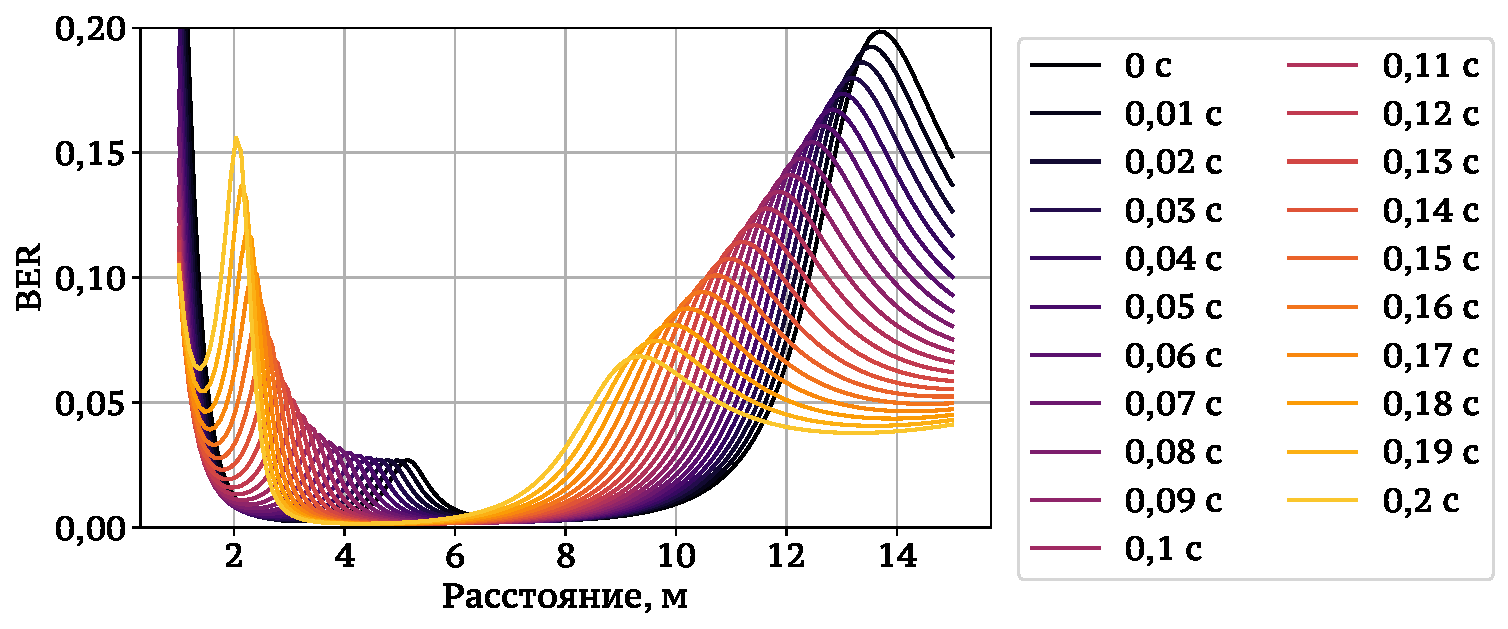
\includegraphics[width=3.3in]{chapter2/ch2_ber_doppler}
  }
	\caption[Зависимость BER от расстояния и времени]{Зависимость вероятности битовой ошибки (BER) от расстояния между считывателем и меткой $d$ и временем, прошедшим с начала приема меткой сигнала от считывателя.}
	\label{fig:ch2_ber_doppler}
\end{figure}



Наличие эффекта Доплера делает канал зависимым от времени (см. \cite{Matz2011}), поскольку, как видно из формулы \eqref{eq:ch2_rx_signal}, величина сдвига для каждого луча определяется индивидуально и зависит от времени, прошедшего с начала получения сигнала. Особенность RFID-системы состоит в том, что считыватель не перестает передавать сигнал (постоянный, который метка может модулировать для передачи своего ответа, или информационный) ни после передачи своей команды, ни после получения ответа. Считыватель может прекращать передачу сигнала, например, для сброса флагов сессий меток, при переключении частот или в том случае, если по законодательству он должен периодически освобождать радиоканал. Однако, такие прерывания происходят относительно редко, внутри одного или нескольких раундов сигнал не прерывается. Поэтому значение $t$ в \eqref{eq:ch2_rx_signal} определяется как время, прошедшее со включения считывателя, за вычетом длительности распространения сигнала от считывателя до метки. Хотя метка в это время может еще находиться далеко, радиоканал уже будет существовать. Учитывая, что в момент включения считывателя метки расположены на разных расстояниях от считывателя, получаем, что значение $t$ в одной и той же точке для разных меток будет разным, а соответственно разными будут и значения $r(t)$. Так, на рис.~\ref{fig:ch2_power_doppler} показана зависимость мощности сигнала, принятой считывателем, от расстояния $d$, измеренного вдоль дороги, а на рис.~\ref{fig:ch2_ber_doppler} "--- зависимость вероятности битовой ошибки (BER) от расстояния $d$. Различные кривиые соответствуют различному времени, прошедшему с начала приема меткой сигнала от считывателя. Графики на рис.~\ref{fig:ch2_heatmap}, \ref{fig:ch2_power_doppler} и \ref{fig:ch2_ber_doppler} показывают, как эффект Доплера делает канал зависимым от времени: области хорошего приема с высоким уровнем принятого сигнала и, соответственно, низким BER, сдвигаются с течением времени.

\begin{figure}[!t]
	\centerfloat{
    \includegraphics[width=3.3in]{chapter2/ch2_pathloss_cases}
  }
	\caption{Зависимости потери при распространении сигнала от расстояния для параллельной, перпендикулярной и круговой поляризаций. Для круговой поляризации комплекснозначный коэффициент равен полусумме коэффициентов для параллельной и перпендикулярной поляризаций.}
	\label{fig:ch2_pathloss_cases}
\end{figure}

На рис.~\ref{fig:ch2_pathloss_cases} показаны результаты расчета затухания сигнала в зависимости от расстояния для разных видов поляризации: параллельной, перпендикулярной и круговой. Различие обусловлено тем, что коэффициент отражения от земли $R_1$ для NLoS-компоненты сигнала принимает разные значения в зависимости от выбранной поляризации (см. рис.~\ref{fig:ch2_reflection}).

Коэффициент отражения определен следующей формулой \cite{Gonzalez2013}:
$$
  R = \frac{\sin\phi - \sqrt{C}}{\sin\phi + \sqrt{C}},
$$
где $\phi$ "--- угол падения, $C = \eta - \cos^2\phi$ для горизонтально поляризованной компоненты и $C = \frac{\eta - \cos^2\phi}{\eta^2}$ для вертикально поляризованной; $\eta = \epsilon_r(f)-j60\lambda\sigma(f)$, где $\epsilon_r(f)$ "--- относительная диэлектрическая проницаемость поверхности для заданной частоты $f$, $\sigma(f)$ "--- проводимость.

\begin{figure}[!t]
	\centerfloat{
    \includegraphics[scale=0.75]{chapter2/ch2_reflection}
  }
	\caption{Зависимость коэффициента отражения от угла падения для параллельной, перпендикулярной и круговой поляризации при разных значениях относительной диэлектрической проницаемости $\epsilon$ и проводимости $\sigma$.}
	\label{fig:ch2_reflection}
\end{figure}

Относительная диэлектрическая проницаемость и проводимость сильно зависят от влажности поверхности. Проводимость меняется в диапазоне от 0.00014~См/м для очень сухой земли до 5~См/м для морской воды. Относительная диэлектрическая проницаемость меняется в диапазоне от 3 до 70. На рис.~\ref{fig:ch2_reflection} показана зависимость коэффициента отражения от угла для разных значений относительной диэлектрической проницаемости $\epsilon$ и проводимости $\sigma$.

Далее будем считать, что у метки простая дипольная антенна, и её диаграмма направленности определяется как:

\begin{equation}\label{eq:ch2_dipole}
	\Gamma(\theta) = \left|
		\frac{\cos{\frac{\pi}{2}\sin{\theta}}}{\cos{\theta}} \right|,
\end{equation}

Для простоты, будем считать, что диаграмма антенны считывателя также определяется с помощью~\eqref{eq:ch2_dipole}. Для более точного расчета можно использовать более подходящие диаграммы, например "--- патч-антенны \cite{Balanis2016}.




%%% --------------------------------------------
\subsection{Расчёт вероятности битовой ошибки (BER)}
%%% --------------------------------------------
\begin{figure}[!t]
	\centerfloat{
    \includegraphics[width=3.3in]{chapter2/ch2_ber_miller}
  }
	\caption{Вероятность битовой ошибки (BER) для разных модуляций ответов метки.}
	\label{fig:ch2_ber_miller}
\end{figure}

Рассмотрим радиоканал с аддитивным гауссовским шумом (AWGN). Вероятность ошибки в передаче бита (BER) можно выразить следующей формулой:

\begin{equation}
	P_{er} = 2Q(\acute{\gamma})[1-Q(\acute{\gamma})],
	\label{eq:ch2_awgn}
\end{equation}
где $Q(\cdot)$ "--- Q--функция; $\acute{\gamma} = mE_s/N_0\cos^2{\phi_s}$; $m$ "--- число символов на бит (порядок) в коде Миллера, $E_s$ "--- энергия одного символа, $N_0/2$ "--- спектральная плотность белого шума и $\phi_s$ "--- разность между реальной и принятой фазами сигнала. Соотношение $E_s/N_0$ может быть выражено как $\gamma T_s B$, где $\gamma$ отношение сигнал-шум (SNR), $T_s$ "--- длительность символа и $B$ "--- ширина полосы.

Для синхронизации фазы передатчик начинает передачу кадра с преамбулы. Ошибка в оценке этой фазы выражается параметром $\phi_s$, который может быть промоделирован с помощью нормально распределенной случайной величины с нулевым средним и дисперсией $\sigma_s^2 = 1/\gamma T_{pr}B$, где $T_{pr}$ "--- длительность преамбулы.

Использование гауссовской модели оказывается слишком оптимистичным, так как при расчете мощности принятого сигнала учитываются не все лучи. Поэтому далее будет использоваться выражением, получаемым усреднением $P_{er}$ в формуле \eqref{eq:ch2_awgn} по $\acute{\gamma}$, которую считаем случайной величиной, имеющей распределение Рэлея \cite{Lazaro2009}:

$$
	P_{er} = \frac{1}{2} - \frac{1}{\sqrt{1+\frac{2}{\acute{\gamma}}}} +
			 \frac{2}{\pi}\frac{\arctan{\sqrt{1+\frac{2}{\acute{\gamma}}}}}{1+\frac{2}{\acute{\gamma}}}.
$$

На рис.~\ref{fig:ch2_ber_miller} показана зависимость BER от выбранного типа кодирования ответа метки. Как и следовало ожидать, при росте числа символов на бит $m$ BER снижается. Влияние эффекта Доплера на BER показано на рис.~\ref{fig:ch2_ber_doppler} и рис.~\ref{fig:ch2_heatmap_ber}. Из-за высокого BER (0.02 и выше) на большей части дороги успешный прием данных от метки практически невозможен, таким образом для передачи данных остаются небольшие <<окна>> шириной 1--2 метра, в которых BER оказывается достаточно низок.







%%%%%%%%%%%%%%%%%%%%%%%%%%%%%%%%%%%%%%%%%%%%%%%%%%%%%%%%%%%%%%%%%%%%%%%%%%%%%%%%
\section{Имитационная модель}\label{sec:ch2_sim}
%%%%%%%%%%%%%%%%%%%%%%%%%%%%%%%%%%%%%%%%%%%%%%%%%%%%%%%%%%%%%%%%%%%%%%%%%%%%%%%%
Для анализа системы радиочастотной идентификации была разработана имитационная модель, позволяющая анализировать производительность системы при разных настройках протокола, учитывающая особенности окружения и интенсивность автомобильного трафика. Имитационная модель позволяет учитывать многолучевое распространение сигнала, эффект Доплера, диаграммы направленности антенн и прочие особенности, описанные ранее. Также имитационная модель содержит детализированную реализацию протокола EPC Gen2, позволяя оценивать производительность системы в зависимости от всевозможных настроек протокола, включая длительности символов, схемы кодирования ответов меток, сценарии управления питанием считывателя и прочее. Модель реализована на языке Python 3. Исходный код и документация доступны на GitHub по адресу https://github.com/larioandr/thesis-models/src/rfidsim.



%%% --------------------------------------------
\subsection{Библиотека дискретно-событийного моделированя PyONS}
%%% --------------------------------------------
Специально для имитационной модели системы радиочастотной идентификации на языке Python 3 была разработана экспериментальная библиотека для дискретно-событийного моделирования PyONS. Исходный код и документация также доступны на GitHub по адресу https://github.com/larioandr/thesis-models/src/pyons. При разработке ставились следующие задачи:

\begin{itemize}
\item возможность написания моделей в функциональном или объектно-ориентированном стиле;
\item обработчики событий, инициализаторы и финализаторы, условия остановки и удаления объектов "--- произвольные функции или методы Python со специальными декораторами;
\item диспетчеризация событий "--- через предикаты, задаваемые в декораторах обработчиков;
\item модели должны содержать минимум <<ритуального кода>>, то есть связывания обработчиков и событий, выполнение инициализаторов и финализаторов и прочие служебные действия должны происходить внутри системы моделирования, и не должны требовать дополнительных вызовов из самих моделей.
\end{itemize}

Состояние системы можно определять либо с помощью произвольного объекта (например, словаря \texttt{dict} или класса данных \texttt{dataclass}), либо с помощью специальных объектов (\textit{сущностей}), унаследованных от класса \texttt{Entity}. В первом случае все управляющие функции задаются с помощью обычных функций Python. Сама модель устанавливается вызовом \texttt{set\_model()} перед началом симуляции и может быть получена из любого обработчика вызовом функции \texttt{get\_model()}. Во втором случае управляющие функции могут также задаваться функциями, но можно их также определять как методы объекта-сущности. После создания, сущности нужно регистрировать в симуляторе вызовом \texttt{add\_entity()}. В любом случае, функции или методы, выполняющие управление моделью, должны снабжаться специальными декораторами.

Сущности модели имеют свой жизненный цикл. После создания они инициализируются, для чего выполняются все методы-инициализаторы, которые в них определены. Затем сущности могут обрабатывать события, пока один из их методов, помеченных как <<условие смерти>>, не вернет \texttt{True}. Если это произойдет, будут выполнены все методы, помеченные как финализаторы, и после этого сущность будет удалена, а все события, которые предназначались ей или отправлены ею, но еще не обработаны, будут отменены. Использование сущностей

Система определяет шесть типов управляющих функций или методов, для которых используются специальные декораторы:

\begin{itemize}
\item \texttt{eventhandler(guard, default, name)} "--- декоратор для обработчиков событий, в который передается предикат (\texttt{guard}), возвращающий True, если событие должно обрабатываться этим обработчиком. Один из обработчиков может быть определен с декоратором, в котором \texttt{default = True}, он будет вызываться, если предикаты всех обработчиков вернули \texttt{False}. Обработчику можно задать удобно читаемое имя (последний параметр декоратора).
\item \texttt{initializer(stage, name)} "--- декоратор для функций или методов, инициализирующих модель. Первый параметр определяет порядок вызова инициализаторов, если их несколько. Смысл инициализатора-функции и инициализатора-метода разный: функция вызывается в начале запуска модели, а метод "--- при создании объекта-сущности.
\item \texttt{finalizer(stage, name)} "--- декоратор для функций, выполняющихся в конце симуляции, или методов, которые выполняются в случае смерти объекта-сущности.
\item \texttt{stop\_condition(guard, name)} "--- декоратор для функций или методов, которые выполняют роль предиката остановки: если одна из таких функций вернет \texttt{True}, симуляция будет остановлена. Для экономии времени, предикаты остановки выполняются не всегда, а только когда функция \texttt{guard} (\textit{страж}, первый аргумент декоратора) возвращает \texttt{True}. Следует отметить, что страж имеет смысл определять только тогда, когда его выполнение занимает меньше времени, чем проверка самого условия остановки.
\item \texttt{death\_condition(guard, name)} "--- декоратор для методов, выполняющих роль условий гибели сущности. Если один из таких методов объекта-сущности вернет \texttt{True}, то сущность погибнет "--- выполнятся все ее методы-финализаторы и она будет удалена из системы. Роль первого аргумента (стража) аналогична его роли в декораторе условий остановки \texttt{stop\_condition(guard, name)}. Условием смерти может быть только метод класса-сущности, для функций вне сущностей он не имеет смысла.
\item \texttt{managed} "--- декоратор без аргументов для методов сущностей. Он не выполняет специфических задач, но его вызов попадает в стек модели.
\end{itemize}

Так как события связываются с обработчиками с помощью предикатов, то код моделей можно организовать по-разному. Например, можно использовать единственную функцию-обработчик в каждой сущности, без предиката-сторожа (\texttt{guard = None}) и установленную по-умолчанию (\texttt{default = True}). Такой же подход используется в OMNeT++, где для обработки событий используется перегружаемая функция \texttt{handleMessage()}. А можно вводить отдельные обработчики для каждого типа событий, и с помощью предикатов определять связи между конкретными событиями и обработчиками.

Система моделирования поддерживает свой собственный стек вызовов, в который попадают управляющие функции и методы. Это позволяет, например, однозначно идентифицировать объект-сущность, метод которого в данный момент выполняется. Это необходимо при создании новых событий, так как в них хранится информация о том, какой обработчик какой сущности это событие создал. Эта информации очень часто нужна для диспетчеризации "--- выбора обработчика для события. Например, событие окончания ожидания ответа должно обрабатывать та же метка, которая его создала.

В ядре модели определно две очереди: очередь будущих запланированных событий и очередь мгновенных вызовов. В качестве очереди будущих событий используется стандартная куча (heap queue) с упорядочиванием по времени наступления событий и, если времена одинаковы, их идентификаторам. Для событий, которые должны наступить в настоящем (то есть фактически для вызова функций-обработчиков, но не из контекста текущего обработчика) используется отдельный массив, чтобы снизить нагрузку на очередь отложенных событий, так как добавление и извлечение событий из нее требует больше времени ($O(1)$ против $O(\log N)$).

Событием в имитационной модели может быть что угодно, включая строки, кортежи, числа, произвольные объекты. Вместе с каждым событием хранятся: его идентификатор, сущность назначения (\texttt{target}, необязательное поле), сущность, которая создала событие (\texttt{source}, необязательное поле) и время наступления события (\texttt{fire\_time}). Для работы с событиями определены три функции:

\begin{itemize}
\item \texttt{create\_timeout(dt, event)} "--- создать событие-таймаут, которое должно наступить через интервал \texttt{dt}, для той же сущности, которая его создает. Если создание происходит не из некоторого метода объекта-сущности, то сущность назначения не будет определена. События, созданные с помощью этого вызова, попадают в очередь будущих событий.
\item \texttt{send\_event(event, entity)} "--- создать событие, которое должно быть обработано указанной сущностью. Это событие попадет в очередь мгновенных событий (то есть массив). Использование \texttt{send\_event} медленнее, чем простой вызов метода объекта-сущности. Однако, во-первых, оно позволяет не указывать явно, какой именно метод нужно вызывать и, во-вторых, вызов соответствующего метода-обработчика произойдет уже после того, как вызывающий обработчик полностью завершится.
\item \texttt{cancel(event\_id)} "--- удалить запланированное, но еще не обработанное событие с заданным идентификатором. Идентификатор возвращается функциями \texttt{create\_timeout()} и \texttt{send\_event()}.
\end{itemize}

Для того, чтобы ядро могло вызывать инициализаторы и финализаторы, находить обработчики событий и проверять условия остановки или смерти сущностей, оно должно знать о них. Декораторы управляющих функций регистрируют их в специальном реестре статических функций \texttt{StaticRegistry}. Так как декораторы выполняются при импорте модуля, то для этого достаточно импортировать файл, в котором определены функции, в модуль, содержащий функцию, вызывающую выполнение модели. Для класса \texttt{StaticRegistry} используется шаблон Singleton, то есть в любой момент времени в системе существует ровно один его объект.

С сущностями ситуация сложнее, так как для вызова метода нужно иметь созданный объект класса-сущности. Для решения этой задачи все классы-сущности используют метакласс \texttt{MetaEntity}, в котором определен аналог реестра статических функций. Конструктор метакласса вызывается при определении класса. Он просматривает все атрибуты класса, находит управляющие методы и записывает их в свой реестр. Этот реестр (фактически, набор спиской  для каждого типа управляющих функций) добавляется к атрибутам создаваемого класса, и далее используется для поиска и итераций по управляющим методам. Для созданных объектов-сущностей используется отдельный реестр \texttt{EntitiesRegistry}, в котором хранятся сущности и информация об их состоянии (только создана, инициализирована, готова к удалению).

Более подробную информацию о реализации PyONS и простые примеры моделей можно найти в документации проекта на GitHub. Основное преимущество реализованной системы моделирования - простота написания моделей, поддержка функциональной и объектно-ориентированной парадигмы программирования, высокая гибкость, а также то, что весь код реализован на Python и может легко интегрироваться с популярными библиотеками работы с числовыми данными "--- NumPy, Pandas, SciPy и другими. Главный же недостаток "--- низкая производительность, которая обусловлена как тем, что вся реализация построена на Python, так и тем, что при обработке каждого события происходит выполнение большого количества служебного кода "--- в первую очередь, поиск нужного обработчика, а также проверка условий остановки и смерти. Возможное решение проблемы с производительностью в перспективе "--- переписать часть ядра на C/C++ и использовать Cython.




%%% --------------------------------------------
\subsection{Модель системы радиочастотной идентификации}
%%% --------------------------------------------
Модель системы радиочастотной идентификации автомобилей построена на базе библиотеки PyONS. Некоторые архитектурные идеи при разработке были заимствованы из библиотеки INET системы моделирования OMNeT++, однако реализованы на Python и с существенными упрощениями, адаптированными для модели RFID.

Модель поддерживает следующие параметры: число полос движения и их ширина, стороны расположения антенн считывателя и меток (передние и/или задние номера), учитывать или нет эффект Доплера, модели расчета затуханий и BER, уровень термического шума и шума в циркуляторе, диэлектрическая проницаемость и проводимость дорожного полотна, угол установки антенн считывателя, смещение по горизонтали и высота подвеса антенн считывателя, высота размещения меток, диаграмма, поляризация и усиление антенн, потери на модуляции (для меток), в кабелях (для считывателя), выходная мощность и частота считывателя, интервалы и длительность сброса питания считывателя, частота обновления положений автомобилей с метками, стратегия выбора флагов сессий, число раундов на каждой антенне, значения Tari, TRcal, RTcal, TRext, M, Q, DR, SL, скорость и длина автомобилей, чувствительность меток, интервалы между появлениями и длительность нахождения в системе автомобилей.

Автомобили появляются в системе через заданные интервалы, причем интервал можно задавать как случайную функцию без аргументов, чтобы сильнее рандомизировать результаты. Скорость движения всех автомобилей одинакова, и через заданное время автомобили исчезают из системы.


В модели определены классы-сущности (наследники класса \texttt{pyons.Entity}):

\begin{itemize}
	\item \texttt{Reader} "--- модель считывателя, которая отвечает за логику создания команд и обработки ответов, периодическое включение и выключение питания, циклическую активизцию антенн;
	\item \texttt{Tag} "--- модель метки, отвечает за логику обработки команд и формирование ответов, а также моделирует включения и отключения при изменении мощности принятого сигнала;
	\item \texttt{Vehicle} "--- модель автомобиля, задача которой "--- периодическое обновление положения связанных с ней меток;
	\item \texttt{Generator} "--- генератор автомобилей, периодически добавляет в систему новые машины;
	\item \texttt{Trasceiver} "--- модель трансивера, отвечающая за прием, обработку и передачу сигналов;
	\item \texttt{Signal} "--- модель сигнала с кадром команды или ответа с заданным приемником и отправителем, хранит текущее значение мощности и обрабатывает события начала и окончания приема;
	\item \texttt{Channel} "--- модель радиоканала, использующаяся трансиверами для расчета затуханий сигнала.
\end{itemize}

Кроме классов-сущностей, есть несколько вспомогательных классов, в которых нет обработки событий, но методы которых используются из сущностей:

\begin{itemize}
	\item \texttt{ReaderDecider}, \texttt{TagDecider} "--- реализуют метод \texttt{decide()}, возвращающий признак того, успешно ли принят сигнал, а также значения максимального BER и минимального SNR. \texttt{TagDecider} возвращает признак успеха, если полученный сигнал был единственным, и он не прерывался, в противном случае сообщает о коллизии. Сигнал на метке считается прерванным, если во время его получения она отключалась из-за снижения мощности ниже порога чувствительности. \texttt{ReaderDecider} также анализирует, был ли сигнал единственным и не прерывался ли он. После этого, если сигнал был непрерывным и он был один, он вычисляет SNR, и по нему находит оценку BER, с помощью которой вычисляет вероятность успешного приема ответа метки. Если случайное число от 0 до 1, оказывается не более, чем найденная вероятность успешного приема, \texttt{ReaderDecider} возвращает признак успеха и вычисленные значения SNR и BER. Во всех иных случаях он возвращает признак ошибки. Значения мощности сигнала в течение его приема, а также признаки прерывания, хранятся в объекте класса \texttt{Signal}, и обновляются при изменении положения метки, ее включении или отключении, а также при сбросе питания считывателя.
	\item \texttt{ReaderAntenna}, \texttt{TagAntenna} "--- классы, описывающие антенны считывателя и метки. В них хранятся характеристики антенн и векторы, описывающие ориентацию антенны в пространстве.
	\item \texttt{Journal} "--- класс, существующий в единственном экземпляре (Singleton), в котором записываются все изменения, происходящие в модели: состояния канала, меток и считывателя, описание прошедших раундов инвентаризации, результаты передачи ответов и прочая информация. Данные из журнала используются в конце симуляции для расчета характеристик модели.
\end{itemize}

Передача кадров по радиоканалу моделируется с помощью сигналов (\texttt{Signal}). Когда считыватель передает кадр с командой меткам, для каждой метки создается свой объект сигнала, а при передаче ответа от метки "--- один сигнал для считывателя. В сигнале записывается список пар <<время, мощность>> для мощностей передачи и приема. Когда изменяется положение метки или выключается считыватель, вычисляется принятая меткой мощность, и она записывается в соответствующие списки в принимаемых и передаваемых меткой сигналах. Записанные значения мощностей приема используются при вычислении значения SNR. События начала и конца приема приходят не трансиверам, а сигналам, а они, в свою очередь, инициируют прием и обработку кадров трансиверами. Начало приема происходит позже начала передачи на величину задержки на распространение сигнала в атмосфере. Для вычисления затухания используется модель канала (\texttt{Channel}).

Таймауты на начало и конец приема сигнала вычисляются при инициализации объекта класса \texttt{Signal}. У сигнала есть несколько состояний: \texttt{INIT} "--- объект не инициализирован, \texttt{STARTED} "--- сигнал инициализирован, прием еще не начался, \texttt{RECEIVING} "--- идет прием, \texttt{FINISHED} "--- прием завершился, но сигнал еще нужен (например, есть конкурирующие сигналы), \texttt{TERMINATED} "--- сигнал больше не нужен. Когда состояние сигнала достигает \texttt{TERMINATED}, он удаляется из системы.

Для вычисления длительности сигналов, выполняется построение кадров команд и ответов и расчет длительностей всех символов и преамбул. Так как для кодирования команд стандарт определяет метод PIE, в модели строятся их представление в виде нулей и единиц. Единственным упрощением является отказ от точного расчета контрольной суммы "--- предполагается, что она состоит поровну из нулей и единиц.

Изменение состояния модели происходит при обработке следующих событий:

\begin{itemize}
	\item наступление момента появления нового автомобиля: в модель добавляется новый автомобиль, располагаемый достаточно далеко, чтобы метки заведомо сразу не включились;
	\item таймаут обновления положений автомобилей: пересчитываются координаты всех автомобилей и их меток, обновляются мощности передаваемых сигналов, метки могут включаться или выключаться, назначается следующее событие обновления положения автомобилей;
	\item таймаут непрерывной работы считывателя "--- считыватель выключается, обновляется мощность на всех сигналах (она становится равной шуму) и метках, метки отключаются;
	\item таймаут включения считывателя: считыватель повышает выходную мощность и начинает раунд инвентаризации, вычисляется новое значение мощности на метках и, если оно превосходит чувствительность, метки включаются;
	\item таймаут межкадрового интервала: считыватель или метка начинают передачу своей команды или ответа соответственно;
	\item таймаут ожидания ответа: считыватель считает, что метка ничего не ответила, и начинает передачу следующей команды;
	\item таймаут начала приема сигнала: сигнал достиг получателя, трансивер начинает его обработку;
	\item завершение приема сигнала: сигнал завершился, трансивер на получателеле принимает решение об успешности приема;
	\item завершение отправки кадра: считыватель начинается отсчет таймаута ожидания ответа.
\end{itemize}

Единственным условием остановки модели является достижение заданного количества сгенерированных автомобилей. Предикат <<смерти>> сущности автомобиля "--- нахождение его в области чтения более заданного времени. Частота обновления положения автомобилей задается в конфигурации, по-умолчанию она равна 100~мс модельного времени, то есть при скорости движения 60~км/ч метка успевает изменить свое положение примерно на 1,67 метра. В общем случае, чем выше скорость, тем чаще стоит обновлять положение меток.

Достоинства разработанной имитационной модели "--- ее высокая точность и возможность управления, относительно простой дизайн. В модель не сложно добавить поддержку новых команд или реализовать альтернативные сценарии опроса. Главное же ограничение "--- высокая вычислительная сложность модели: так как команды и ответы достаточно короткие, а частота обновления положений автомобилей высока, приходится обрабатывать огромное количество событий, причем при обработке событий приходится вычислять оценки мощностей сигналов и BER, что требует времени. Из-за зависимости затухания от времени со включения считывателя функцию затухания тяжело кэшировать, и приходится производить много вычислений. В результате на получение численных результатов нужно много времени. Например, моделирование проезда 100 автомобилей на скорости 20~м/с с интервалом обновления положения каждые 100~мс на ноутбуке под управлением macOS с процессором Core i7-6920HQ занимает 2 минуты. Для более высокой точности и для вычисления на большом объеме входных данных нужно гораздо больше времени. Все представленные в диссертационном исследовании результаты были получены за несколько часов на многоядерном сервере.






%%%%%%%%%%%%%%%%%%%%%%%%%%%%%%%%%%%%%%%%%%%%%%%%%%%%%%%%%%%%%%%%%%%%%%%%%%%%%%%%
\section{Результаты имитационного моделирования}\label{sec:ch2_results}
%%%%%%%%%%%%%%%%%%%%%%%%%%%%%%%%%%%%%%%%%%%%%%%%%%%%%%%%%%%%%%%%%%%%%%%%%%%%%%%%
В ходе численного эксперимента были получены оценки идентификации мобильных меток и автомобилей, на которых метки были установлены. При этом автомобиль считался идентифицированным, если была успешно прочитана хотя бы одна метка. Кроме того, для более глубокого понимания работы системы, было исследовано число раундов, в которых успевает принять участие движущаяся метка.



%%% --------------------------------------------
\subsection{Анализ влияния частоты переключений антенн на число раундов}
%%% --------------------------------------------
Точное число раундов, в которых успевает принять участие метка, зависит как от настроек протокола (схема кодирования ответов метки, выбор параметра Q и пр.), так и от алгоритма выбора сессии и частоты смены антенн. Так как вероятность прочитать и EPCID, и TID в одном раунде относительно мала, существенным оказывается то, в скольких раундах метка успевает принять участие, т.е. сколько у нее будет попыток передать свои идентификаторы.

В начале раунда инвентаризации считыватель выбирает сессию (S0, S1, S2, S3) и значение её флага ($A$ или $B$). Метка отвечает только в том случае, если хранимеый ею флаг выбранной сессии совпадает с переданным в команде Query. После рассылки своего EPCID в ответе на ACK, метка инвертирует значение хранимого флага сессии ($A \rightarrow B,\, B \rightarrow A$). Для каждой сессии стандарт определяет интервал времени после выключения питания, в течение котрого метка должна сохранять значение флага сессии, а после которого, если питания так и не появилось, "--- возвращать значение $A$. В дальнейшем будем рассматривать сессию S0, для которой эта процедура самая прстая "--- значение $A$ должно быть установлено сразу после сброса питания, независимо от длительности длительности потери энергии.

\begin{figure}[!t]
	\centerfloat{
    \includegraphics[width=3.6in]{chapter2/ch2_rounds_per_tag}
  }
	\caption{Число раундов, в которых участвует метка, в зависимости от длительности работы на одной антенне, для разных стратегий выбора флага сессии.}
	\label{fig:ch2_rounds_per_tag}
\end{figure}

Если считыватель использует одну антенну без периодического выключения питания, число раундов, в которых участвует метка, зависит только от стратегии выбора флага сессии. На рис.~\ref{fig:ch2_rounds_per_tag} приведены результаты симуляции, которые показывают, что число раундов при опросе меток только со значением флага сессии S0=$A$ (самая нижняя горизонтальная линия) и число раундов при смене значений запрашиваемых флагов каждый раунд отличаются в шесть раз. В первом случае число раундов, в которых принимает участие метка, определяется только числом включений метки (выключения обусловлены приемом сигнала считывателя на уровне, меньшем чувствительности метки). При периодической смене флагов метка имеет возможность повторно участвовать в опросе и без выключения, поэтому число раундов оказывается значительно больше, а тем самым повышается вероятность того, что хотя бы один раз метка успешно передаст свои идентификационные данные. Небольшие колебания на приведенном графике обусловлены случайным характером процесса чтения меток, а также случайностью длительности раундов, зависящей от числа занятых и пустых слотов. Также следует отметить, что на число раундов может влиять выбор параметра Q (график соответствует значению Q=2), а также использование операции Select, которая в представленном исследовании не использовалась.

Если считыватель использует несколько антенн и периодически между ними переключается, число раундов также зависит от интервала между переключениями антенн. На рис.~\ref{fig:ch2_rounds_per_tag} показаны результаты, полученные исходя из того, что считыватель размещен над однополосной дорогой и оборудован двумя антеннами, направленными в противоположные стороны (для чтения переднего и заднего номеров). Можно видеть, что периодическая смена флагов сессии также позволяет увеличить число раундов, хотя и меньше, чем при использовании одной антенны. Можно заметить, что сильнее всего выбор интервала переключения антенн влияет на число раундов при малых значениях интервала. Это связано, в первую очередь, с тем, что при этом переключение происходит каждый раунд или быстрее, метка может не успеть передать свой EPCID до потери энергии (здесь предполагается, что переключение антенн не связано с границами раунда, что является некоторым упрощением). Это связано, в первую очередь, с тем, что периоды работы на одной антенне быстро становятся сопоставимыми с длительностью проезда зон с уровнем сигнала от считывателя, превышающим чувствительность меток. При увличении мощности сигнала или чувствительности меток зависимость должна оказываться более сильной.

Следует отметить, что при использовании других сессий (например, S2), результаты оказываются ближе к случаю отсутствия переключения антенн для малых интервалов, так как при малых интервалах между переключениями (меньших, чем время сохранения флага сессии) метка может <<не заметить>> потерю энергии и сохранить значение флага.

На число раундов также влияет длительность работы считывателя до его выключения и время нахождения в выключенном состоянии. Все расчёты в этом и следующем разделе сделаны в предположении, что считыватель выключается каждые 2 секунды на 100 милисекунд.



%%% --------------------------------------------
\subsection{Анализ вероятности идентификации транспортных средств}
%%% --------------------------------------------
С помощью имитационной модели была изучена вероятность идентификации меток, расположенных на номерах автомобилей, двигающихся по однополосной дороге. Считыватель был оборудован двумя антеннами, размещенными над дорогой в противоположных направлениях, для чтения переднего и заднего знаков.

Для выбора параметра Q было рассчитано среднее число меток, участвующих в одном раунде. Результаты этого расчета приведены в табл.~\ref{table:ch2_tags_num_per_round}, где $N_v$ "--- среднее число автомобилей вблизи считывателя, $T_v$ "--- средний интервал времени между появлениями автомобилей, $N_t$ "--- среднее число меток, участвующих в раунде, а $N_t^{(1)}$ "--- среднее число меток в тех раундах, в которых участвует хотя бы одна метка. Из приведенных результатов видно, что даже при очень интенсивном потоке, когда в зоне действия считывателя оказывается более пяти машин, из-за неравномерности уровня сигнала большая часть меток оказывается выключенными, и можно считать, что в каждом раунде участвует не более одной метки. Фактически это означает, что вероятностью коллизий можно пренебречь и выбирать значение Q сколь угодно малым, так как его увеличение лишь добавит пустых слотов. Учитывая, что длительность пустого слота достаточно мала и для перестраховки на тот случай, когда помимо меток в номерех в зону действия попадут  другие метки (расположенные, например, на предметах под стеклом автомобиля или на самом автомобиле), можно установить Q=2. В дальнейшем это значение будет использовано для получения остальных результатов.

\begin{table}[!t]
	\renewcommand{\arraystretch}{1.3}
	\caption{Среднее число меток, участвующих в раунде, при движении автомобилей со скоростью 60~км/ч.}
	\label{table:ch2_tags_num_per_round}
	\centering
	\begin{tabular}{|c|c|c|c|}
		\hline
		$T_v$, sec & $N_v$ & $N_t$ & $N_t^{(1)}$ \\\hline
		0.5 & 5.67 & 0.1000 & 1.0 \\\hline
		1.0 & 3.38 & 0.0357 & 1.0 \\\hline
		\end{tabular}
\end{table}


\begin{figure}[!t]
  \centerfloat{
    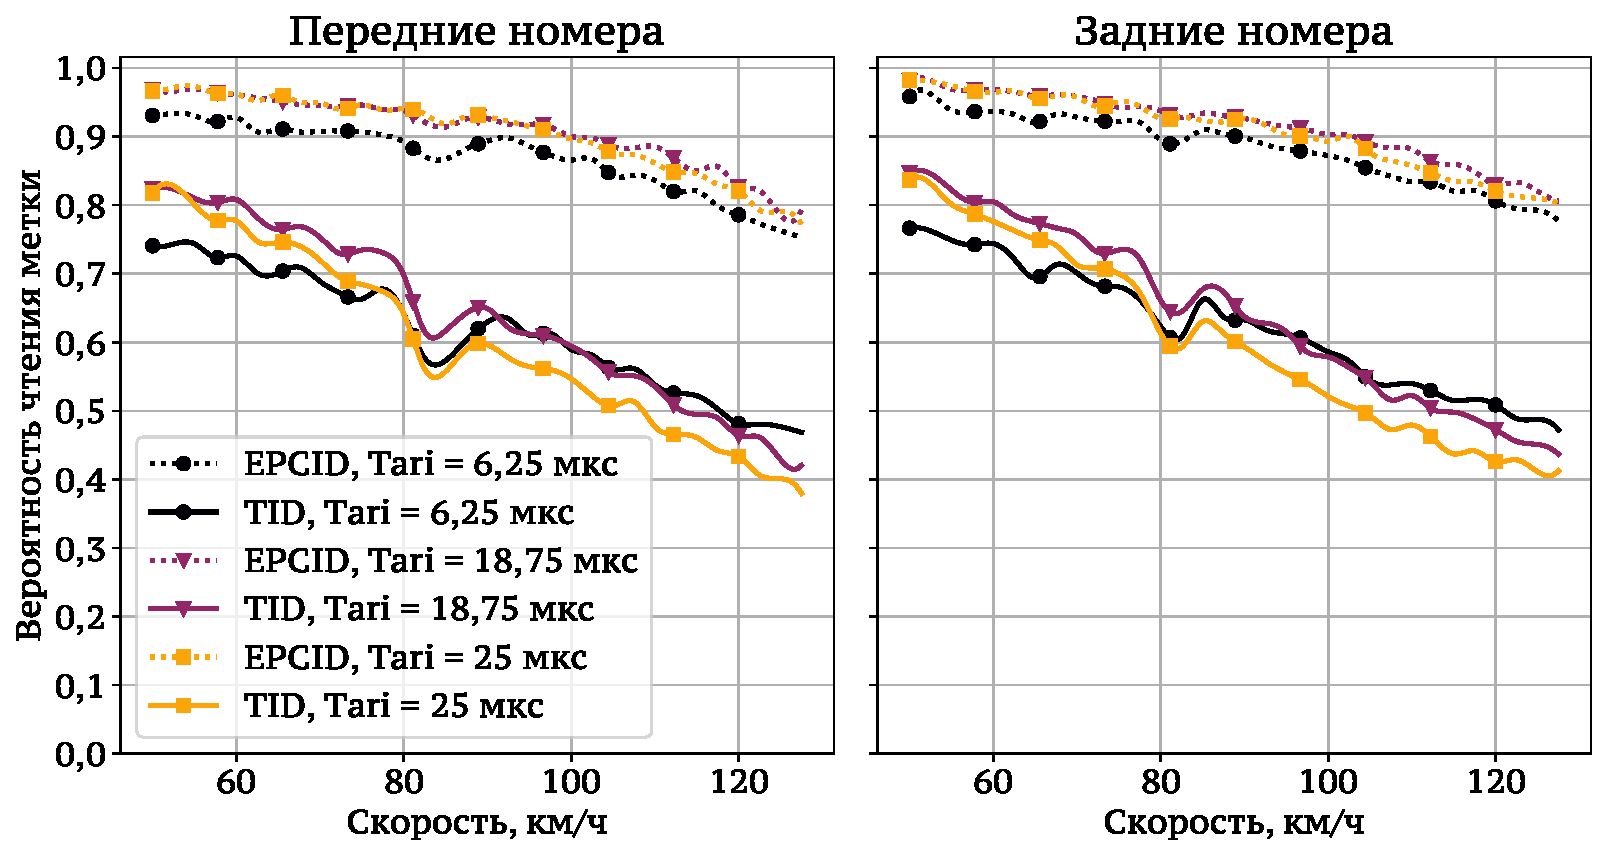
\includegraphics[width=3.3in]{chapter2/ch2_tag_identification_m4}
  }
	\caption{Вероятность успешного чтения меток в номерах при различных значениях Tari и кодировании ответов M=4.}
	\label{fig:ch2_tag_identification_m4}
\end{figure}

\begin{figure}[!t]
  \centerfloat{
    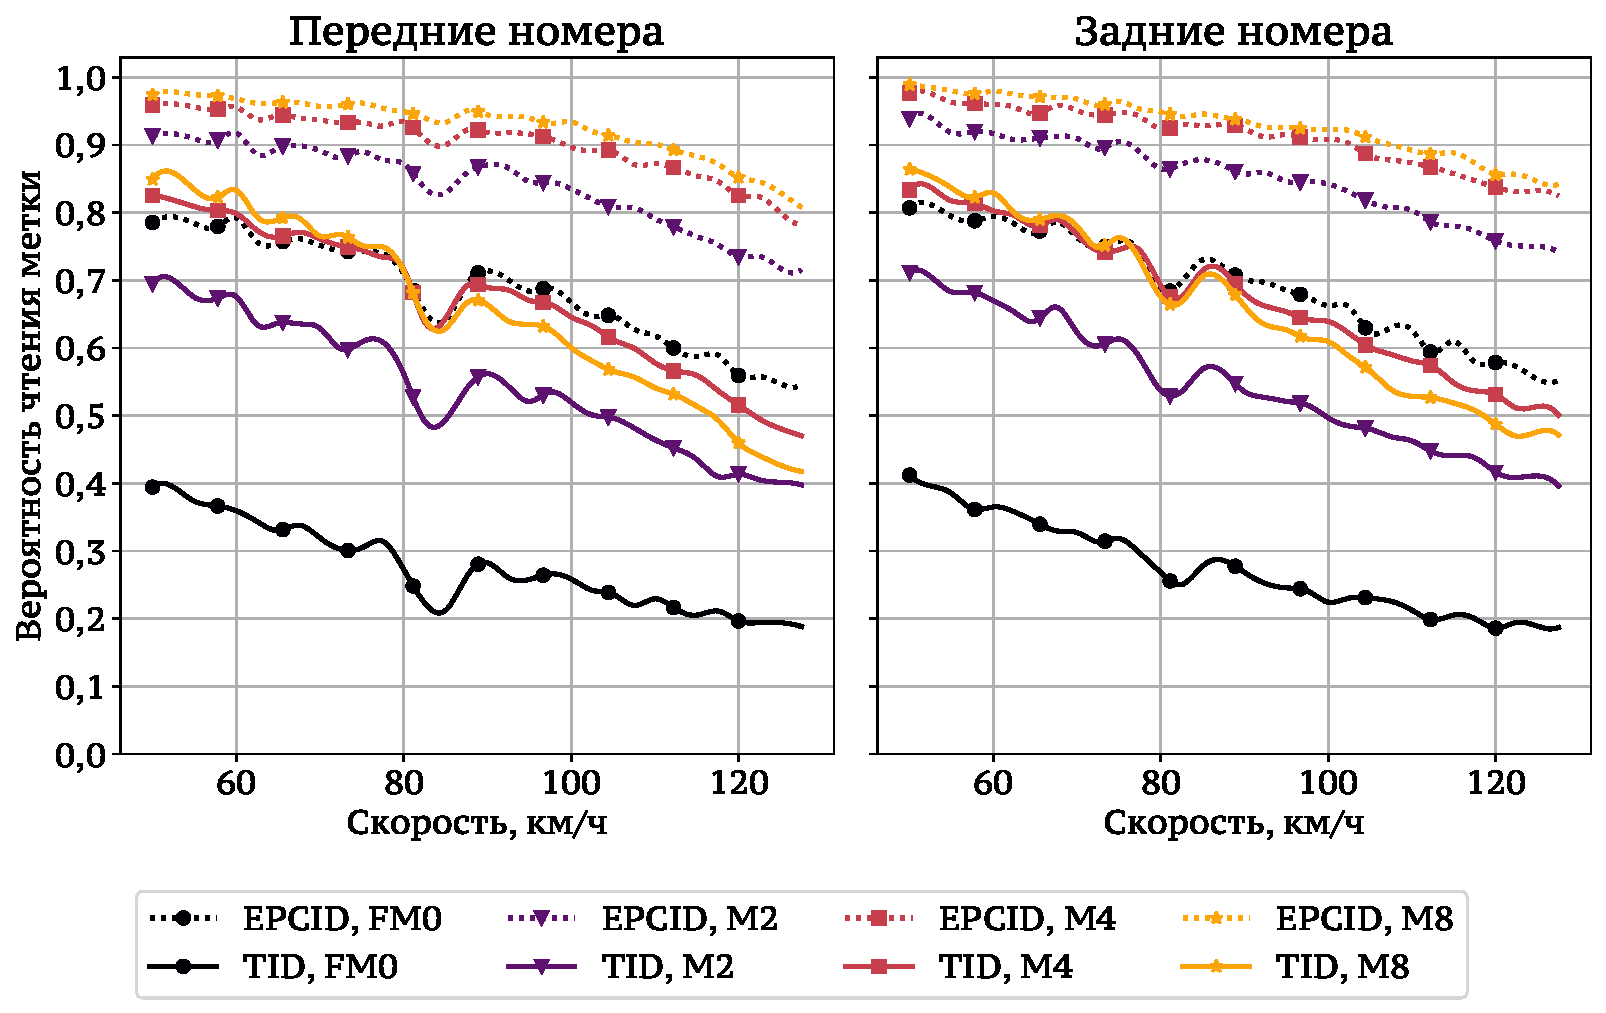
\includegraphics[width=3.3in]{chapter2/ch2_tag_identification_tari125}
  }
	\caption{Вероятность успешного чтения меток в номерах при различных значениях M и Tari = 12,5~мкс.}
	\label{fig:ch2_tag_identification_tari125}
\end{figure}

На рис.~\ref{fig:ch2_tag_identification_m4} и \ref{fig:ch2_tag_identification_tari125} показаны результаты расчёта вероятности идентификации меток в номерах в заивисимости от скорости движения автомобилей при различных значениях интервала Tari (см. рис.~\ref{fig:ch2_tag_identification_m4}) и различных значениях M (число символов на бит в ответах меток, см. рис.~\ref{fig:ch2_tag_identification_tari125}). Предполагалось, что антенны считывателя имеют усиление 8~дБи, потери в кабеле составляют 2~дБ, метки используют расширенные преамбулы, а значение DR=8. Считыватель работал в сессии S0, инвертировал значение флага сессии в каждой команде Query и переключал антенны каждые 100~мс. Из приведенных графиков видно, что вероятность чтения меток падает с ростом скорости. При этом вероятность чтения EPCID остаётся высокой при достаточно больших скоростях свыше 120~км/ч, чего нельзи сказать про чтение TID. Важно отметить, что выбор больших значений Tari не обязательно ведет к увеличению вероятности успешной идентификации (см. рис.~\ref{fig:ch2_tag_identification_m4}), также как и выбор больших значений M (см. рис.~\ref{fig:ch2_tag_identification_tari125}). Более того, при чтении TID выбор самых больших значений Tari=25~мкс и M=8 даёт результаты хуже, чем выбор менее надёжных значений Tari=18,75~мкс и M=4, хотя выбор еще меньших значений также снижает вероятность успешного чтения. Объяснить эту закономерность можно тем, что выбор слишком больших значений ведёт к увеличению длительности раундов и, как следствие, снижению вероятности успешной идентификации хотя бы в одном раунде, хотя и повышает вероятность успешного чтения TID в одном раунде. Дальнейшее же уменьшение значений M и Tari ведет к слишком сильному уменьшению вероятности успешной передачи в одном раунде. Этот вывод подтверждается также тем, что выбор оказывается менее существенным при чтении только EPCID, так как и увеличение длительности раунда там оказывается менее значительным, и влияние вероятности успешной передачи ответов метки меньше зависит от BER (так как в этом случае ответов, которые должна передать метка, в два раза меньше).

\begin{figure}[!t]
  \centerfloat{
    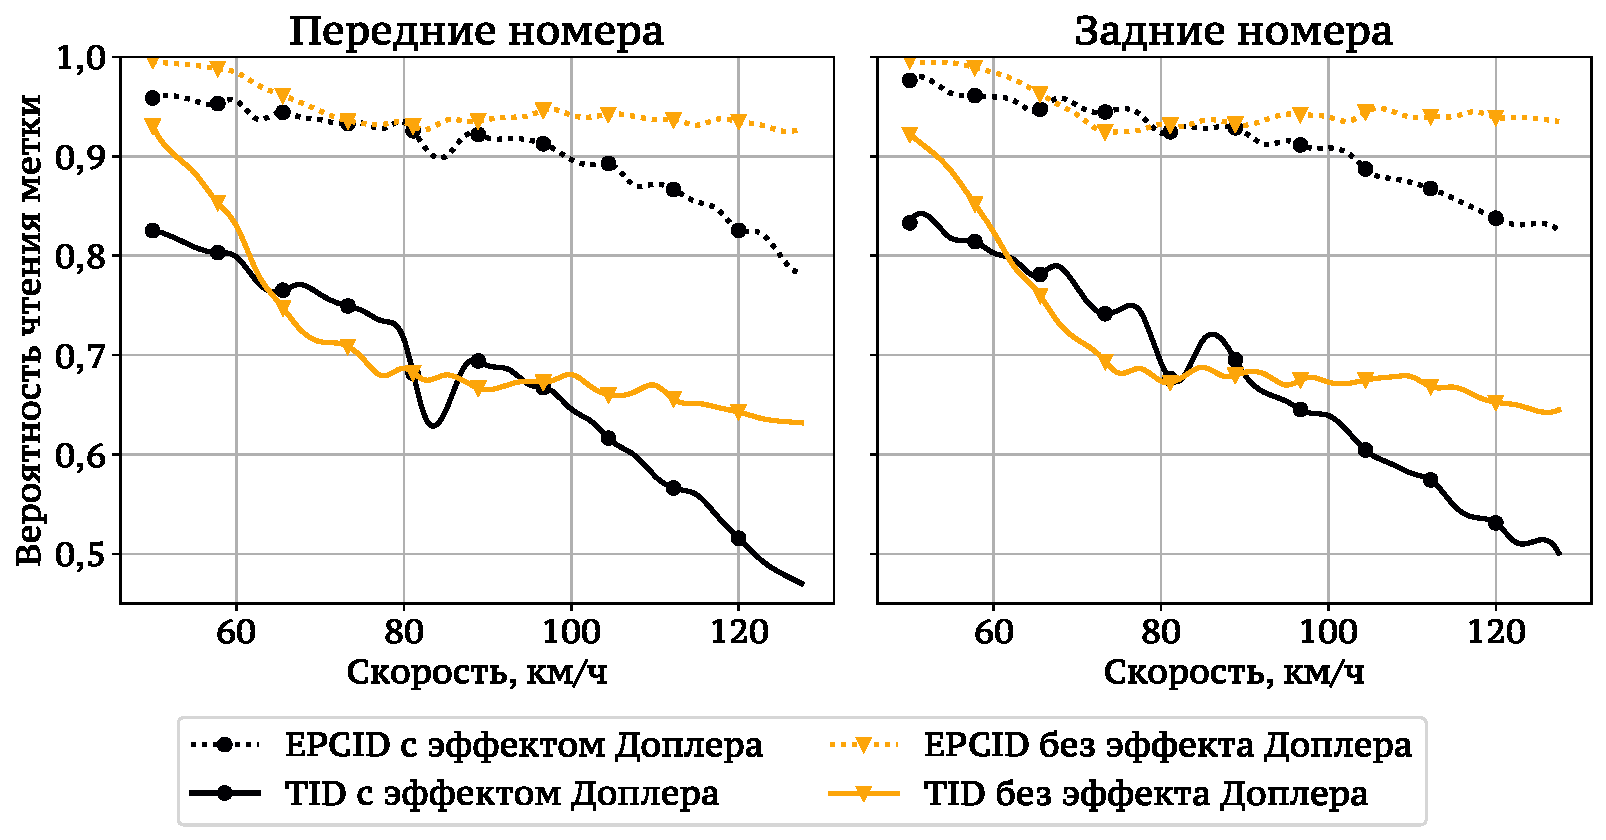
\includegraphics[width=3.3in]{chapter2/ch2_identification_doppler}
  }
	\caption{Влияние эффекта Доплера на вероятность успешного чтения метки при M=4, Tari=12,5~мкс.}
	\label{fig:ch2_identification_doppler}
\end{figure}

Также было проведено численное исследование влияния эффекта Доплера, см. рис.~\ref{fig:ch2_identification_doppler}. Как видно из приведённых результатов, эффект Доплера оказывает существенное влияние на вероятность чтения меток, особенно при чтении TID на высоких скоростях "--- в этом случае эффект Доплера может снижать вероятность успешного чтения метки на 10--20~\%.

\begin{figure}[!t]
	\centerfloat{
    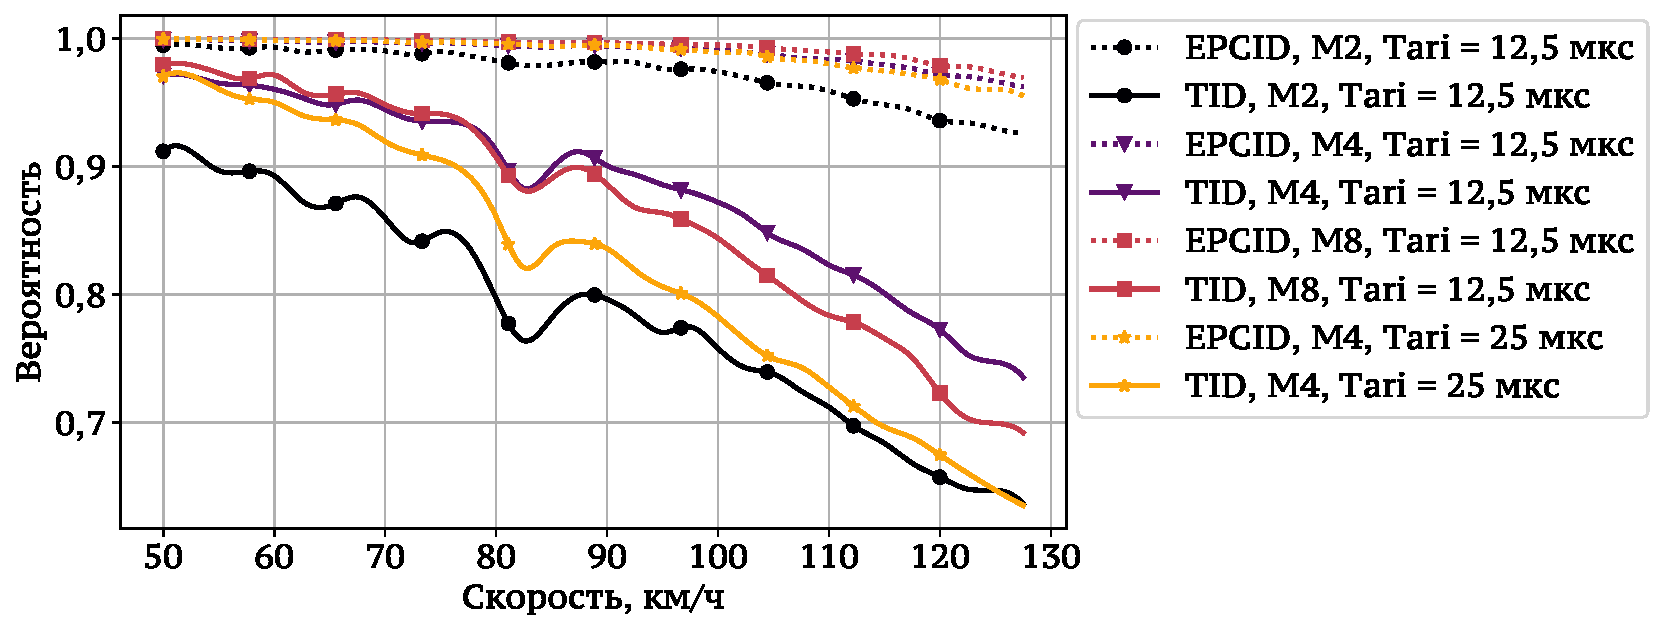
\includegraphics[width=3.2in]{chapter2/ch2_vehicle_identification_rate}
  }
	\caption{Вероятность идентификации автомобиля с метками на переднем и заднем номере, идентифицируемого по любой из меток.}
	\label{fig:ch2_vehicle_identification_rate}
\end{figure}

Результаты расчета вероятности идентификации автомобилей показаны на рис.~\ref{fig:ch2_vehicle_identification_rate}. При проведении расчётов считалось, что автомобиль может быть идентифицирован по любой метке, т.е. для успешной идентификации было достаточно единожды прочитать метку в переднем или заднем номере. Полученные результаты сопадают с данными, полученных в ходе эксперимента в городе Казань (см. главу 5), в котором использовалось значение M=4 и Tari=12,5~мкс, а вероятность идентификации составила около 92--95\%, в зависимости от точки идентификации, при идентификации меток по EPCID и TID. Из приведенных результатов видно, что эти значения дают наилучшую вероятность идентификации быстро движущихся автомобилей. Также можно видеть, что значения M=8 и Tari=25~мкс дают хорошие результаты на небольшой скорости, но затем сильно деградируют и на высоких скоростях дают вероятность, близкую к случаю использования гораздо менее надежных параметров M=2 и Tari=12,5~мкс. Как отмечалось ранее, это связано с тем, что при высоких скоростях длительность раунда становится слишком большой и у метки остаётся мало шансов передать свои идентификаторы.



%%%%%%%%%%%%%%%%%%%%%%%%%%%%%%%%%%%%%%%%%%%%%%%%%%%%%%%%%%%%%%%%%%%%%%%%%%%%%%%%
\section{Заключение}\label{sec:ch2_conclusion}
%%%%%%%%%%%%%%%%%%%%%%%%%%%%%%%%%%%%%%%%%%%%%%%%%%%%%%%%%%%%%%%%%%%%%%%%%%%%%%%%
В главе были представлены следующие результаты:
\begin{enumerate}
	\item описан способ построения системы радиочастотной идентификации автомобилей, рассмотрены основные особенности такой системы и, на основе анализа протокола радиочастотной идентификации EPC Gen2, выделены факторы, влияющие на её производительность;
	\item предложена имитационная модель, учитывающая сценарии идентификации автомобилей (идентификация только по значению EPCID или по паре EPCID и TID), параметры протокола EPC Gen2 (длительности символов в командах считывателя, способы кодирования ответов меток, выбор сессий и значений их флагов, число слотов в раунде), настройки считывателя (периодичность смены антенн и отключения питания), а также особенности распространения сигналов (многолучевое распростренение, зависимость коэффициента отражения от материала дорожного покрытия, эффект Доплера);
	\item с помощью имитационной модели были получены зависимости вероятности идентификации как отдельных номеров, так и автомобилей, от скорости движения, а также от выбранных настроек протокола EPC Gen2.
\end{enumerate}

\FloatBarrier
